% !TEX program = xelatex
\documentclass[12pt]{article}
% 在 Overleaf 中编译时，请使用 \usepackage{ctex}，并删去 [fontset=windows]
\usepackage{ctex}
\usepackage{amsmath}
\usepackage{graphicx}
\usepackage{float}
\usepackage{booktabs}
\usepackage{geometry}
\geometry{a4paper, margin=2cm}

\title{\Huge \textbf{实验一 小信号调谐放大器}}
\author{专业：微电子科学与技术专业 \quad 学号：24308172 \quad 姓名：王钰铖}
\date{}

\begin{document}

\maketitle

\section*{一. 实验目的}
\begin{enumerate}
    \item 熟悉电子元器件和高频电子线路实验系统；
    \item 掌握单调谐和双调谐放大器的基本工作原理；
    \item 掌握测量放大器幅频特性的方法；
    \item 熟悉放大器集电极负载对单调谐和双调谐放大器幅频特性的影响；
    \item 了解放大器动态范围的概念和测量方法。
\end{enumerate}

\section*{二. 实验内容概要}

\vspace{1em}\noindent{\large \textbf{1. 实验原理概述：}}
\begin{itemize}
    \item \textbf{单调谐放大器}：利用单一LC谐振回路作为晶体管放大器的集电极负载。
    
       由于LC回路具有频率选择性，它对谐振频率 $f_0 = \frac{1}{2\pi\sqrt{LC}}$ 的信号具有最强的放大作用（此时回路等效并联谐振阻抗 $R_p$ 达到最大，对应的电压放大倍数 $A_{v0} \approx g_m R_p$ 达到峰值），而对偏离 $f_0$ 的信号放大作用迅速减弱。
     
       回路的有载品质因数 $Q$ 决定了其通频带宽度 $BW_{0.707} = \frac{f_0}{Q}$，即 $Q$ 值越高，频带越窄，选择性越好。
    \item \textbf{双调谐回路放大器}：具有两个调谐回路，一个是晶体管输出端（初级），一个是下级输入端（次级），两者通过耦合电容（如本实验中的 $1C19$）耦合。
    
           通过调节互感或电容大小改变耦合系数，双调谐在临界耦合或相近状态下，能够实现顶部平坦、边缘陡峭的频率响应曲线。它的矩形系数 $K_{R0.1} = \frac{BW_{0.1}}{BW_{0.707}}$ 相比单调谐更接近于 1，从而在保证带宽的同时有效提高了对外带干扰的抑制能力。
    \item \textbf{放大器动态特性}：“小信号”放大的基本前提是输入信号必须足够微弱（通常为几毫伏量级），以确保晶体管仅工作在伏安转移特性曲线的线性放大区间内。
    
    当输入信号幅度逐渐增大并超出这一个线性范围边界时，由于三极管固有特性的非线性，管子工作点将会受推压而进入饱和区或截止区。
    
    宏观物理表现为：输出波形不再是纯正弦波而是开始发生“波形削顶”或底部平坦等非线性大信号失真，此时放大器的电压放大倍数 $A_v$ 也将随着本期输入幅度的增加而急剧下降。
    
    动态范围的检测实质上正是为了精准标定放大器能够保持线性恒增益且不发生波形畸变的“最大输入信号幅度”容忍边界。
\end{itemize}

\vspace{1em}\noindent{\large \textbf{2. 核心实验内容：}}
\begin{enumerate}
    \item[(1)] \textbf{采用点测法测量单调谐和双调谐放大器的幅频特性}：保持输入信号幅度不变，逐点改变输入信号的频率，利用示波器测量输出电压幅度，从而绘制出电压幅值随频率变化的幅频特性曲线。
    \item[(2)] \textbf{用示波器测量输入、输出信号幅度，并计算放大器的放大倍数}：在谐振点读取输入和输出峰峰值，计算 $A = U_{out} / U_{in}$。
    \item[(3)] \textbf{用示波器观察耦合电容对双调谐回路放大器幅频特性的影响}：调整耦合电容 $1C19$ 的大小（改变耦合度），观察双调谐幅频特性峰值及双峰凹陷程度的变化。
    \item[(4)] \textbf{用示波器观察放大器的动态范围}：固定频率在谐振点，逐渐增大输入信号幅度，观察输出波形从正常到失真过程，并计算放大倍数的变化。
    \item[(5)] \textbf{观察集电极负载对放大器幅频特性的影响}：通过开关（如带/不带集电极并联电阻 ）改变集电极等效负载阻抗，观察其对回路品质因数 $Q$ 值、增益及带宽的影响。
\end{enumerate}

\section*{三. 具体实验}

\subsection*{任务一：单调谐放大器幅频特性测量}

操作系统使1K2开关接通（对应指示灯点亮），此时电容1C19被短路，放大器即处于单调谐回路状态。将高频信号源接入放大器输入端1P1，同时使用示波器CH1通道连接输入端测点1TP2以监测输入信号，CH2通道接输出端测点1TP7以观测放大后的输出信号。将高频信号源频率设定为 6.3MHz，并调节使输入信号幅度（峰峰值）保持在 200mV 左右，随后细致调节可变电容电压控制旋钮1W1和1W2，直到示波器CH2通道显示的输出波形幅度达到最大值，这表明放大器回路已谐振于 6.3MHz，此时记录并计算中心频点的放大倍数。

在完成谐振点校准后，进入幅频特性的点测阶段：严格保持 200mV 的输入幅度不变，按照既定的表格步长旋转频率旋钮改变高频源的输入频率，逐点读取并记录对应的输出电压幅度。最后，为了观察负载对电路特性的影响，可通过接通或断开开关1K1，使得电阻1R25并入或脱离开集电极回路，重复测定幅频曲线，仔细对比两种状态下电路输出带宽和电压增益发生的变化规律。

\subsubsection*{1. 测试结果}

\textbf{a. 以下为扫频法的测试结果：}

% 请在这里插入扫频仪截图
\begin{figure}[H]
\centering
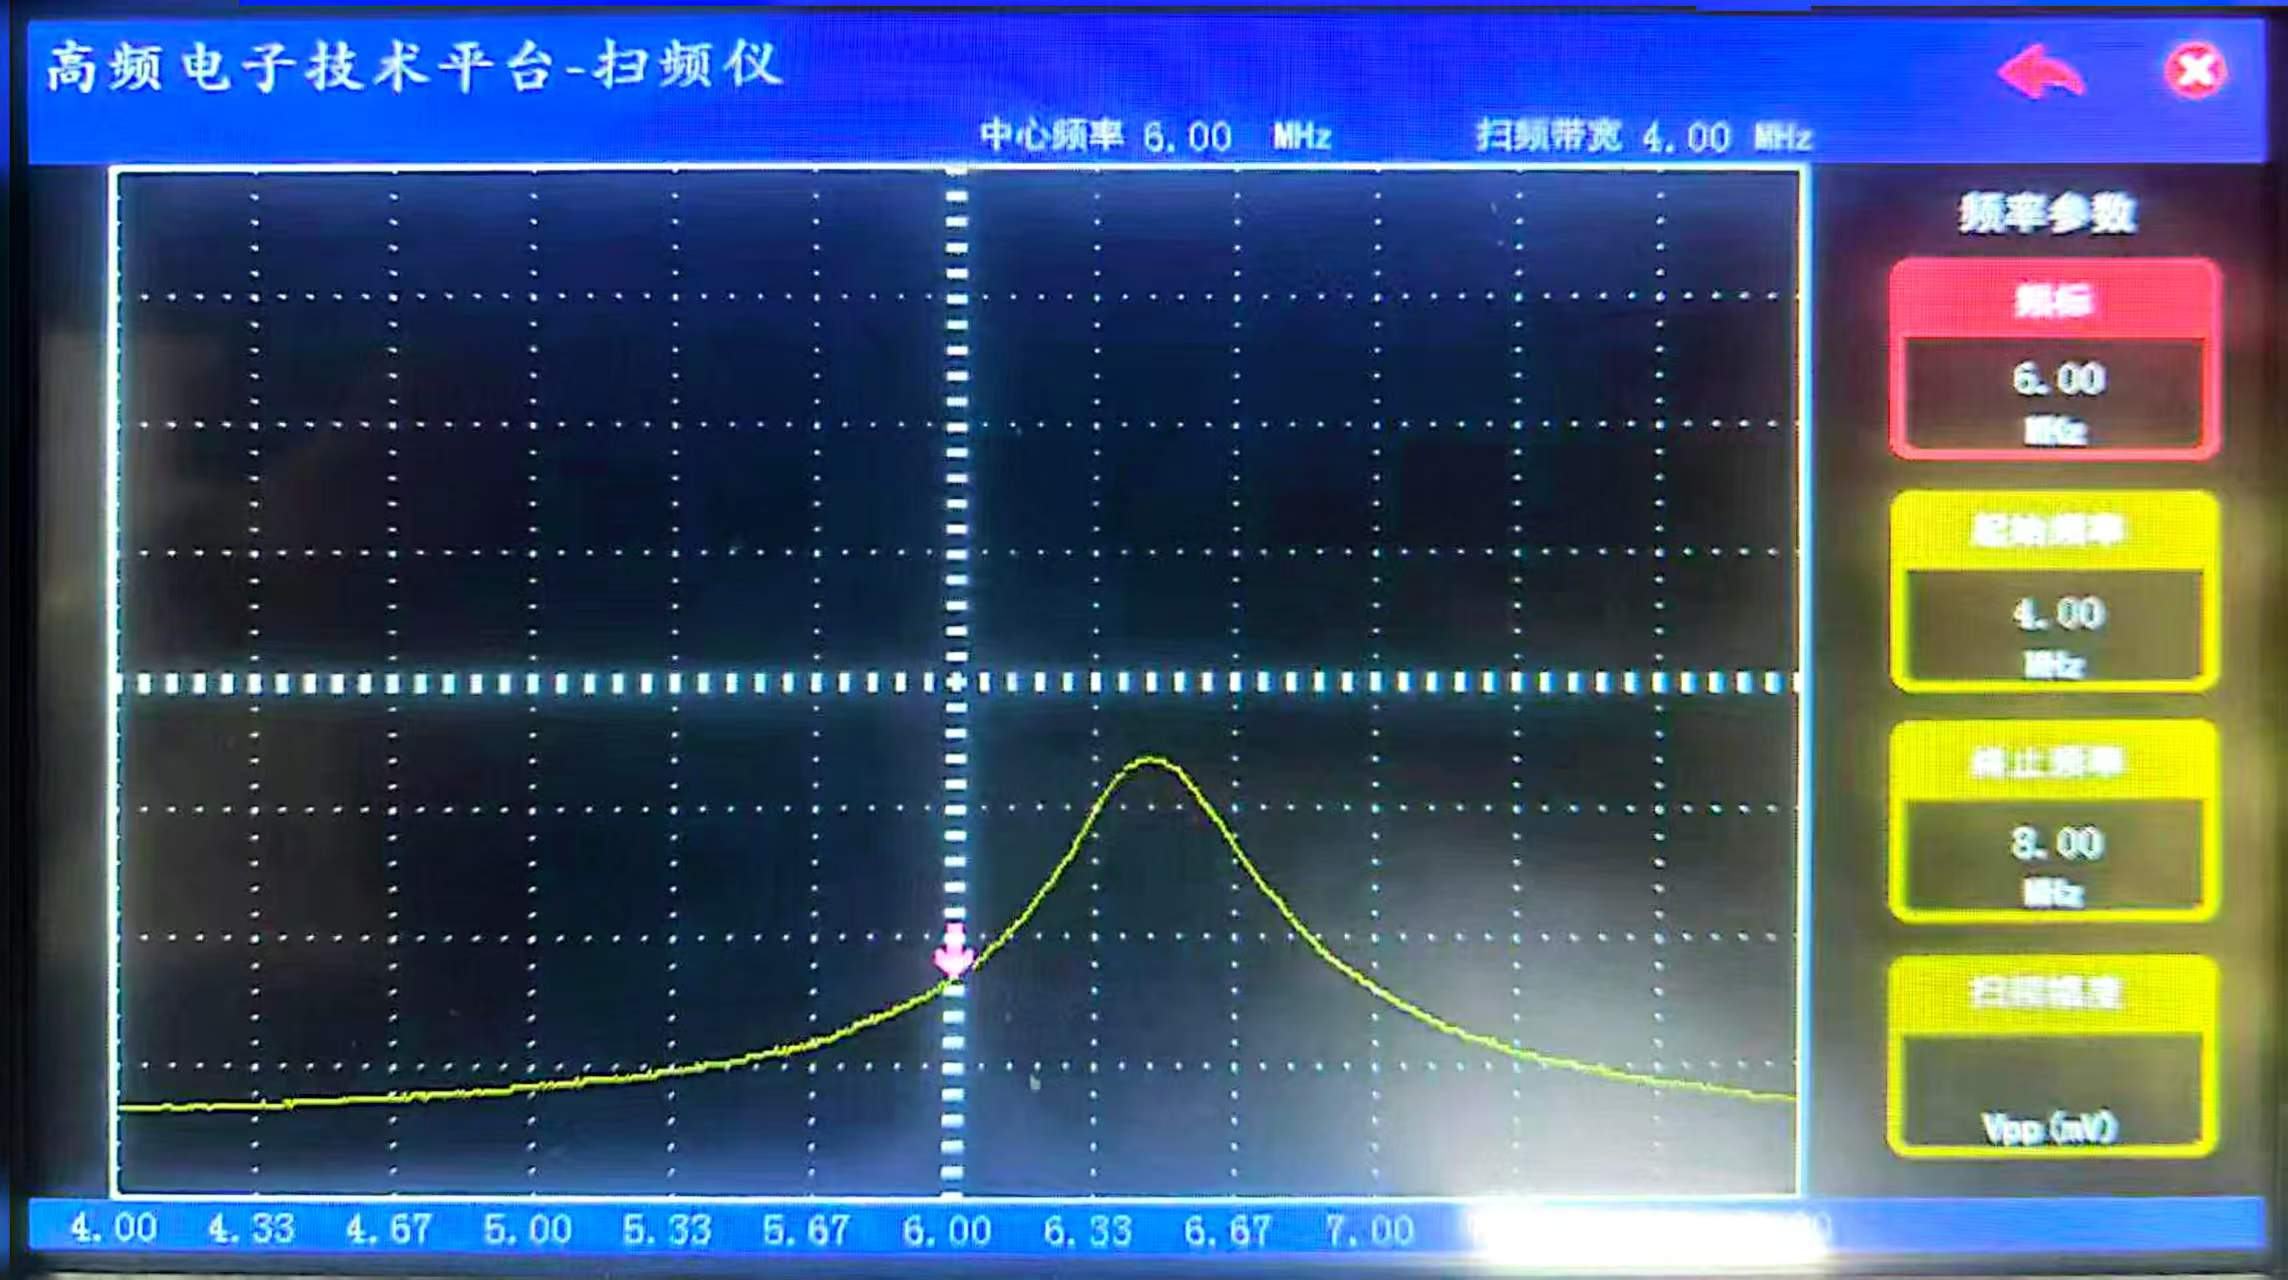
\includegraphics[width=0.8\textwidth]{单调谐扫频法截图.jpg}
\caption{扫频法测得的单调谐放大器幅频特性}
\label{fig:sweep_freq_result}
\end{figure}

\textbf{b. 示波器输出结果：}
\begin{figure}[H]
\centering
\includegraphics[width=0.8\textwidth]{单调谐示波器截图.png}
\caption{单调谐示波器截图}
\label{fig:sweep_freq_result}
\end{figure}


\textbf{c. 以下为点测法的测试结果及单调放大器的幅频特性曲线：}

% 提示：输入信号幅度为 200mV，调整1W1和1W2使输出最大
\begin{table}[H]
    \centering
    % 使用 \makebox[宽度][居中方式]{内容}
    \makebox[\textwidth][c]{
        \begin{tabular}{c*{14}{c}}
        \toprule
        输入频率 $f$ (MHz) & 5.0 & 5.2 & 5.4 & 5.6 & 5.8 & 6.0 & 6.2 & 6.3 & 6.5 & 6.7 & 6.9 & 7.1 & 7.3 & 7.5 \\
        \midrule
        输出幅度 $U_{o}$ (mV) & 424 & 520 & 660 & 920 & 968 & 1020 & 936 & 880 & 600 & 440 & 312 & 256 & 216 & 184 \\
        \bottomrule
        \end{tabular}
    }
    \caption{单调谐放大器幅频特性测试结果}
\end{table}

\begin{figure}[H]
\centering
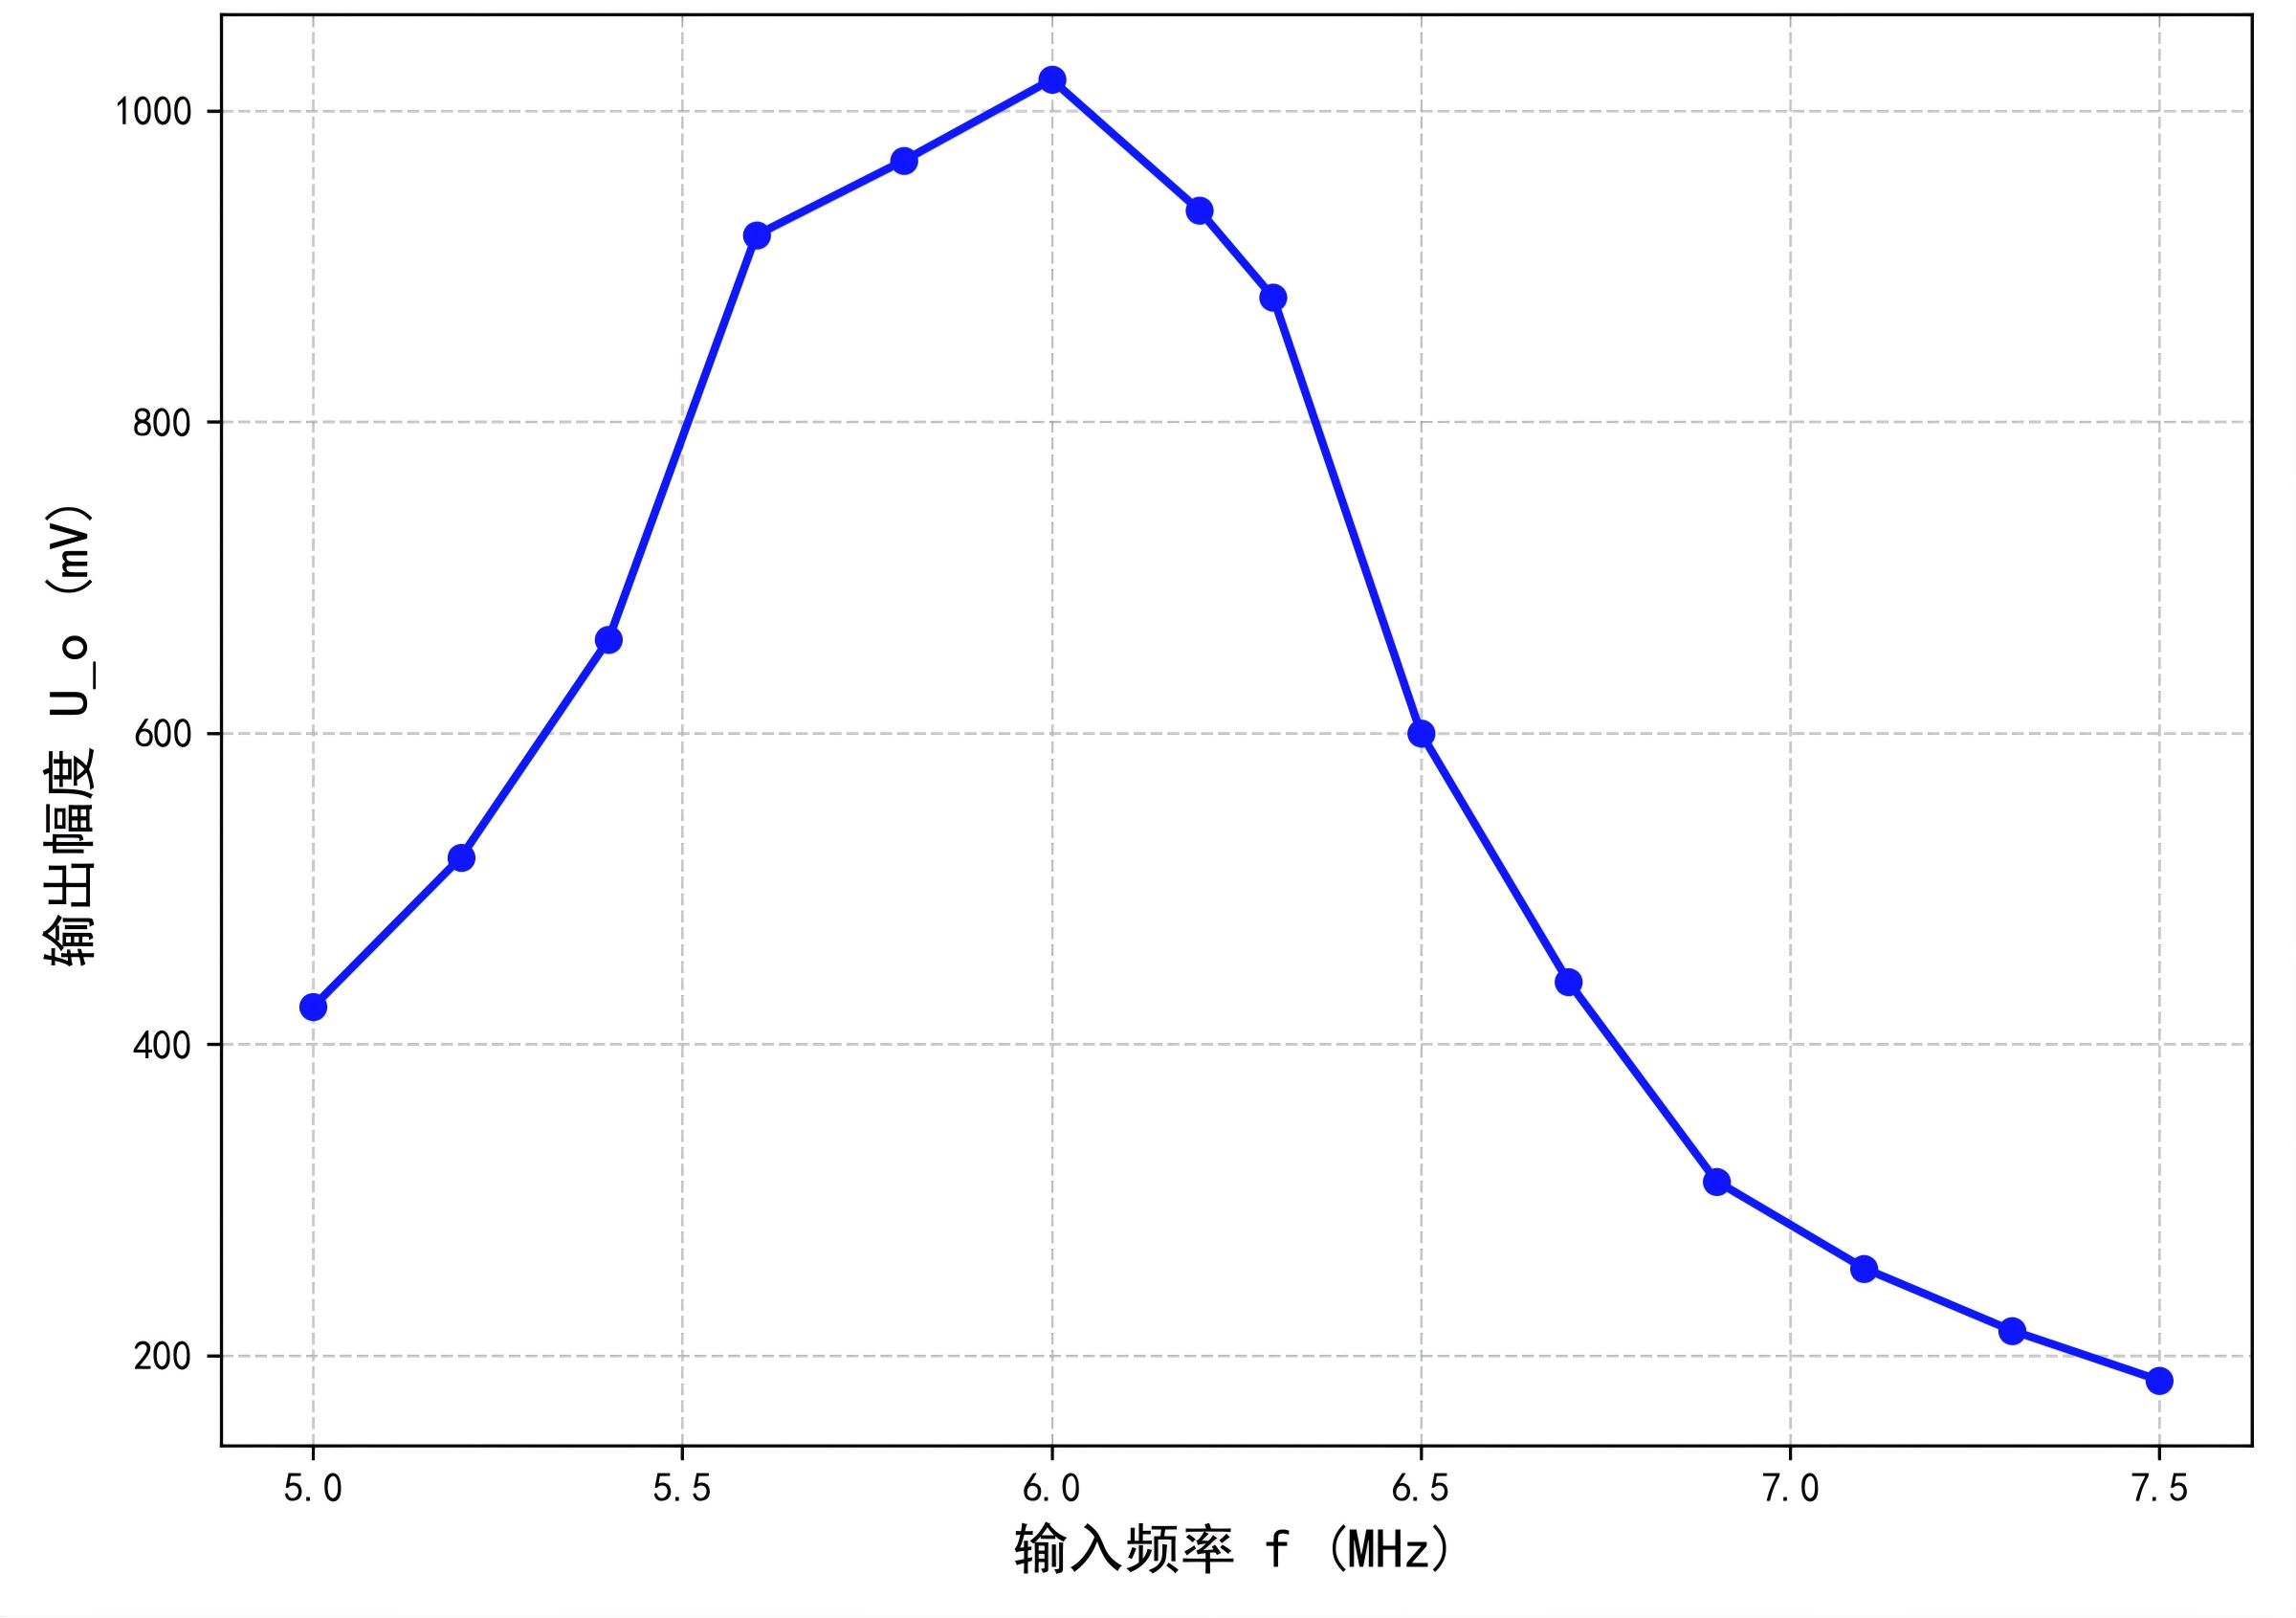
\includegraphics[width=0.8\textwidth]{单调谐幅频特性曲线.png}
\caption{单调谐放大器幅频特性曲线}
\label{fig:single_tuned_curve}
\end{figure}

\subsubsection*{2.结果分析}

% 提示：通过绘制出的曲线，分析放大器的选择性和通频带情况。计算幅值从最大值下降到 0.707 时的带宽。
\textbf{测试数据与通频带分析：}
\begin{itemize}
    \item \textbf{单调谐幅频特性：} 从测试数据可知，当输入信号频率处于 $6.0\text{MHz}$ 时，输出电压达到最大值 $1.02\text{V}$（即 $1020\text{mV}$）。这说明实际装配电路的中心频率（谐振点）偏移至约为 $6.0\text{MHz}$，幅频曲线在此处呈现峰值，向两侧逐步衰减，表现出典型的钟形频率选择性。
    \item \textbf{通频带计算：} 幅值从最大值下降到 $0.707$ 时的基准值为 $1020 \times 0.707 \approx 721\text{mV}$。查表并估算可得左右对应此幅值范围的下限频率 $f_L \approx 5.48\text{MHz}$，上限频率 $f_H \approx 6.38\text{MHz}$。由此计算处放大器的通频带 $BW_{0.707} = f_H - f_L \approx 0.9\text{MHz}$。
\end{itemize}

\subsection*{任务二：观察集电极负载对单调谐放大器幅频特性的影响}

\subsubsection*{1. 测试结果}

\begin{figure}[H]
    \centering
    \begin{minipage}[b]{0.48\textwidth}
        \centering
        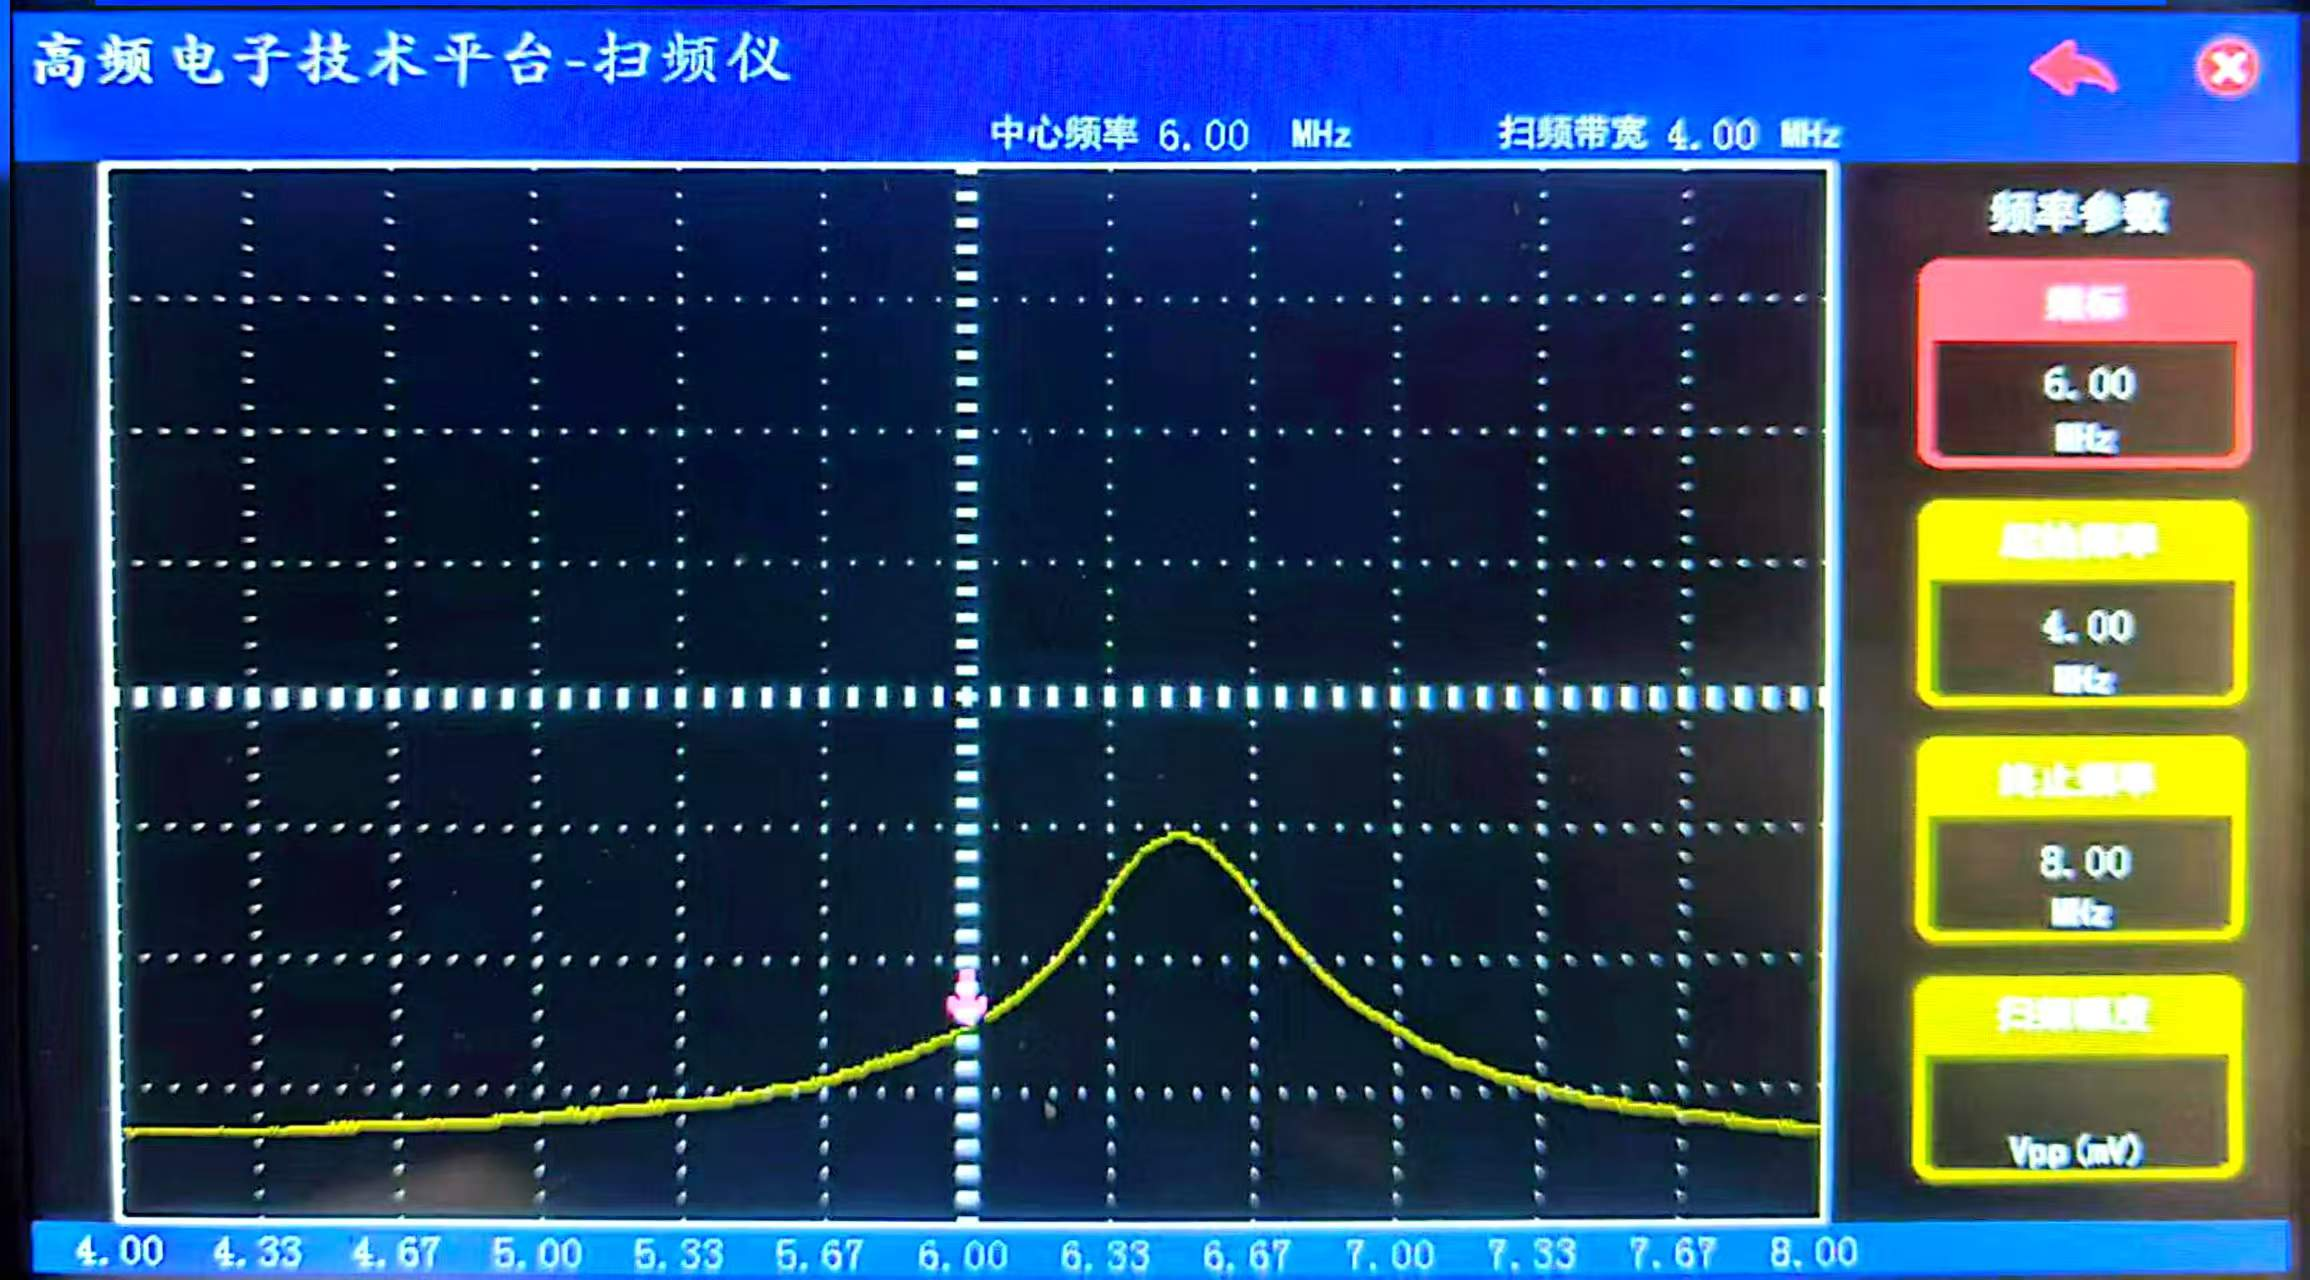
\includegraphics[width=\textwidth, height=3.5cm]{断开负载时的特性曲线.jpg} % 请在此处替换为左侧图片路径
        \caption{断开负载时的特性曲线}
    \end{minipage}
    \hfill
    \begin{minipage}[b]{0.48\textwidth}
        \centering
        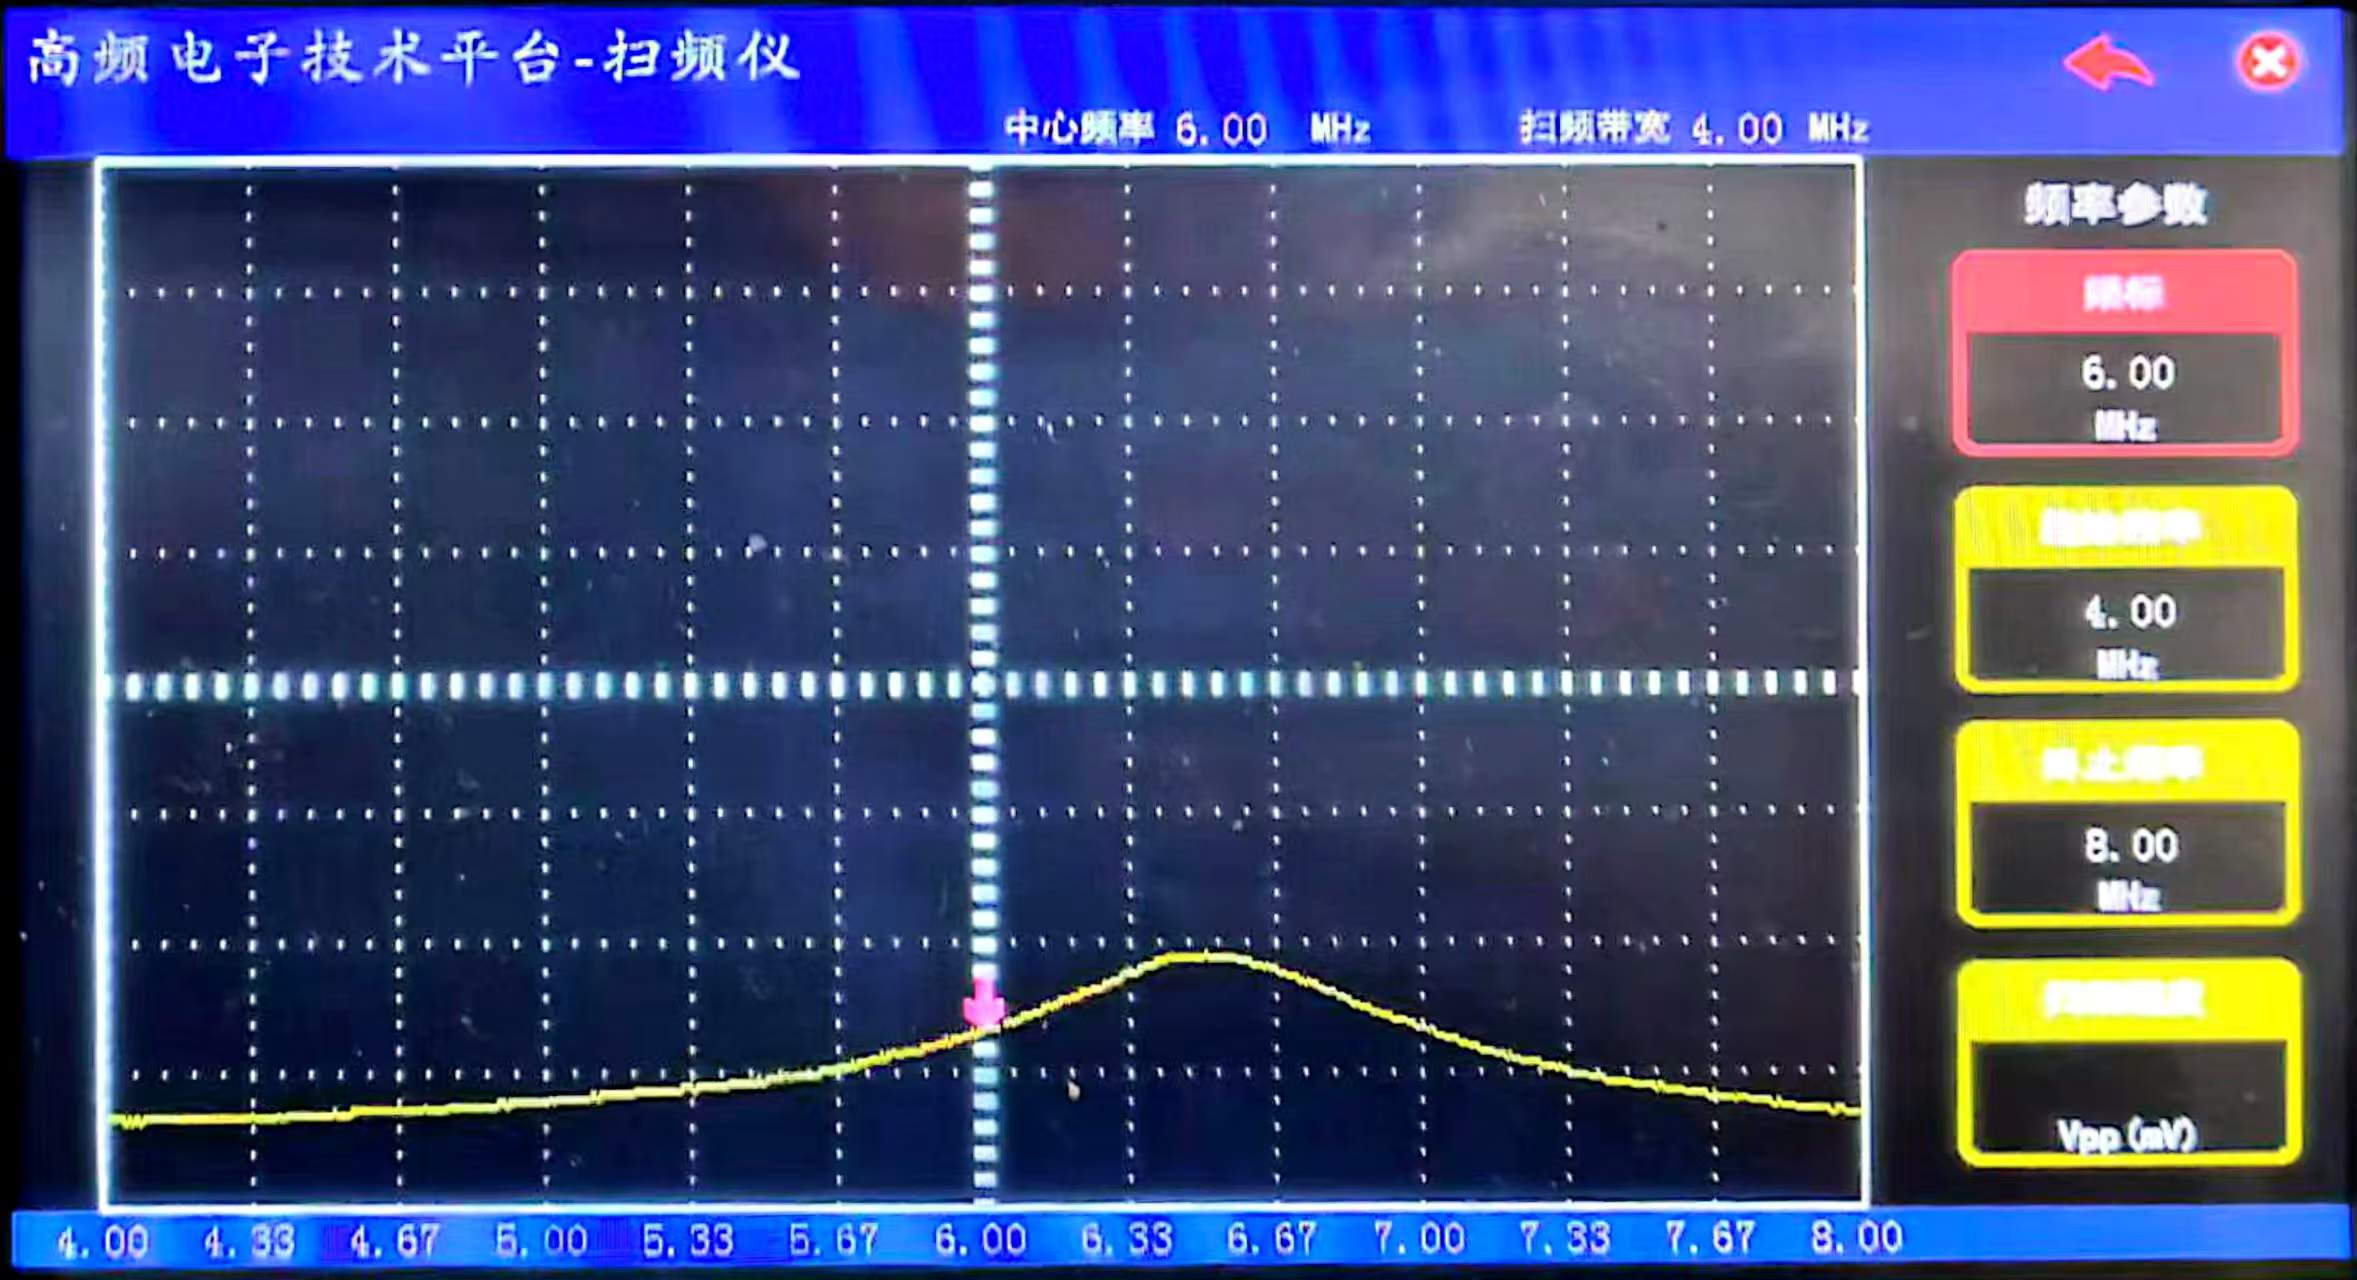
\includegraphics[width=\textwidth, height=3.5cm]{接入负载时的特性曲线.jpg} % 请在此处替换为右侧图片路径
        \caption{接通负载时的特性曲线}
    \end{minipage}
    \vspace{0.5em}
    \label{fig:single_tuned_curve}
\end{figure}

\subsubsection*{2. 结果分析}
\begin{itemize}
    \item \textbf{有载品质因数与通频带的关系：} 当接通开关并入负载电阻时，集电极等效负载电阻减小。根据谐振回路原理，有载品质因数 $Q$ 值极速下降。这将直观地导致幅频特性曲线变“胖”，即通频带 $BW$ 展宽。
    \item \textbf{增益变化：} 由于等效并联谐振阻抗 $R_p$ 的减小，处于中心谐振点时的最大电压增益 $A_{v0}$ 亦随之显著下降。反之，当断开负载电阻时，曲线变“瘦”（选择性增强，通频带变为狭窄），同时中心最大增益上升。这充分从工程上验证了单调谐电路中“增益-带宽”本质上互相制约的经典特性规律。
\end{itemize}

\subsection*{任务三：双调谐回路谐振放大器幅频特性测量}

在进行双调谐回路测试前，将开关1K2置为“断开”状态（对应指示灯熄灭），此时由于耦合电容1C19不再被短路而被接入电路，初次级回路发生耦合，放大器转为双调谐回路工作模式，同时确认开关1K1保持断开。

仪器连接方式与单调谐实验保持一致。将高频源频率调节为6.3MHz，并将其初始输出幅度（由CH1监测）设定在200mV。测量过程与单调谐类似，要求在测试全程保持200mV的输入幅度恒定，按照给定的频率表格逐步改变输入频率，记录每次频率变化对应的输出电压幅度，在点测过程中需特别留意观察和寻找双调谐特性曲线中典型的“双峰”现象以及两峰之间的频率凹陷点。

此外，为了探究耦合度对放大器幅频特性的核心影响，实验中还需要进一步调整电容1C19的容值大小，重新进行该范围内的扫频测试过程，仔细记录并观察由于耦合程度改变所带来的双峰高度拉伸以及中心频率凹陷程度的剧烈差异变化。

\subsubsection*{1. 测试结果}

a. 改变高频信号源的频率，保持高频信号源输出幅度峰-峰值为 200mV（示波器 CH1 监视），从示波器 CH2 上读出与频率相对应的双调谐放大器的幅度值。扫频法输出结果及收集到的数据如下：



\begin{table}[H]
    \centering
    % 第一段：5.4 到 6.0 MHz
    \begin{tabular}{c*{7}{c}}
    \toprule
    输入频率 $f$ (MHz) & 5.4 & 5.5 & 5.6 & 5.7 & 5.8 & 5.9 & 6.0 \\
    \midrule
    \textbf{输出幅度 $U_{o}$ (mV)} & 356 & 544 & 896 & 1032 & 1024 & 1024 & 1016 \\
    \bottomrule
    \end{tabular}

    \vspace{1em} % 两段表格之间的间距

    % 第二段：6.1 到 6.7 MHz
    \begin{tabular}{c*{7}{c}}
    \toprule
    输入频率 $f$ (MHz) & 6.1 & 6.2 & 6.3 & 6.4 & 6.5 & 6.6 & 6.7 \\
    \midrule
    \textbf{输出幅度 $U_{o}$ (mV)} & 1000 & 1000 & 1008 & 1016 & 1024 & 1032 & 1032 \\
    \bottomrule
    \end{tabular}
    \caption{双调谐放大器幅频特性测试结果}
    \label{tab:double_tuned_results}
\end{table}

\begin{itemize}
    \item[b.] \textbf{凹陷点频率测量}：根据测试数据观察，两峰之间的凹陷点大致出现在 $6.15\text{MHz}$ 附近，此时输出幅度约为 $1000\text{mV}$。
    \item[c.] \textbf{幅频特性曲线绘制}：按照表 1-2 数据，双调谐放大器呈现出顶部较为平坦且边缘陡峭的特性，矩形系数明显优于单调谐放大器。
    % 📝 插入刚画好的双调谐曲线
    \begin{figure}[H]
    \centering
    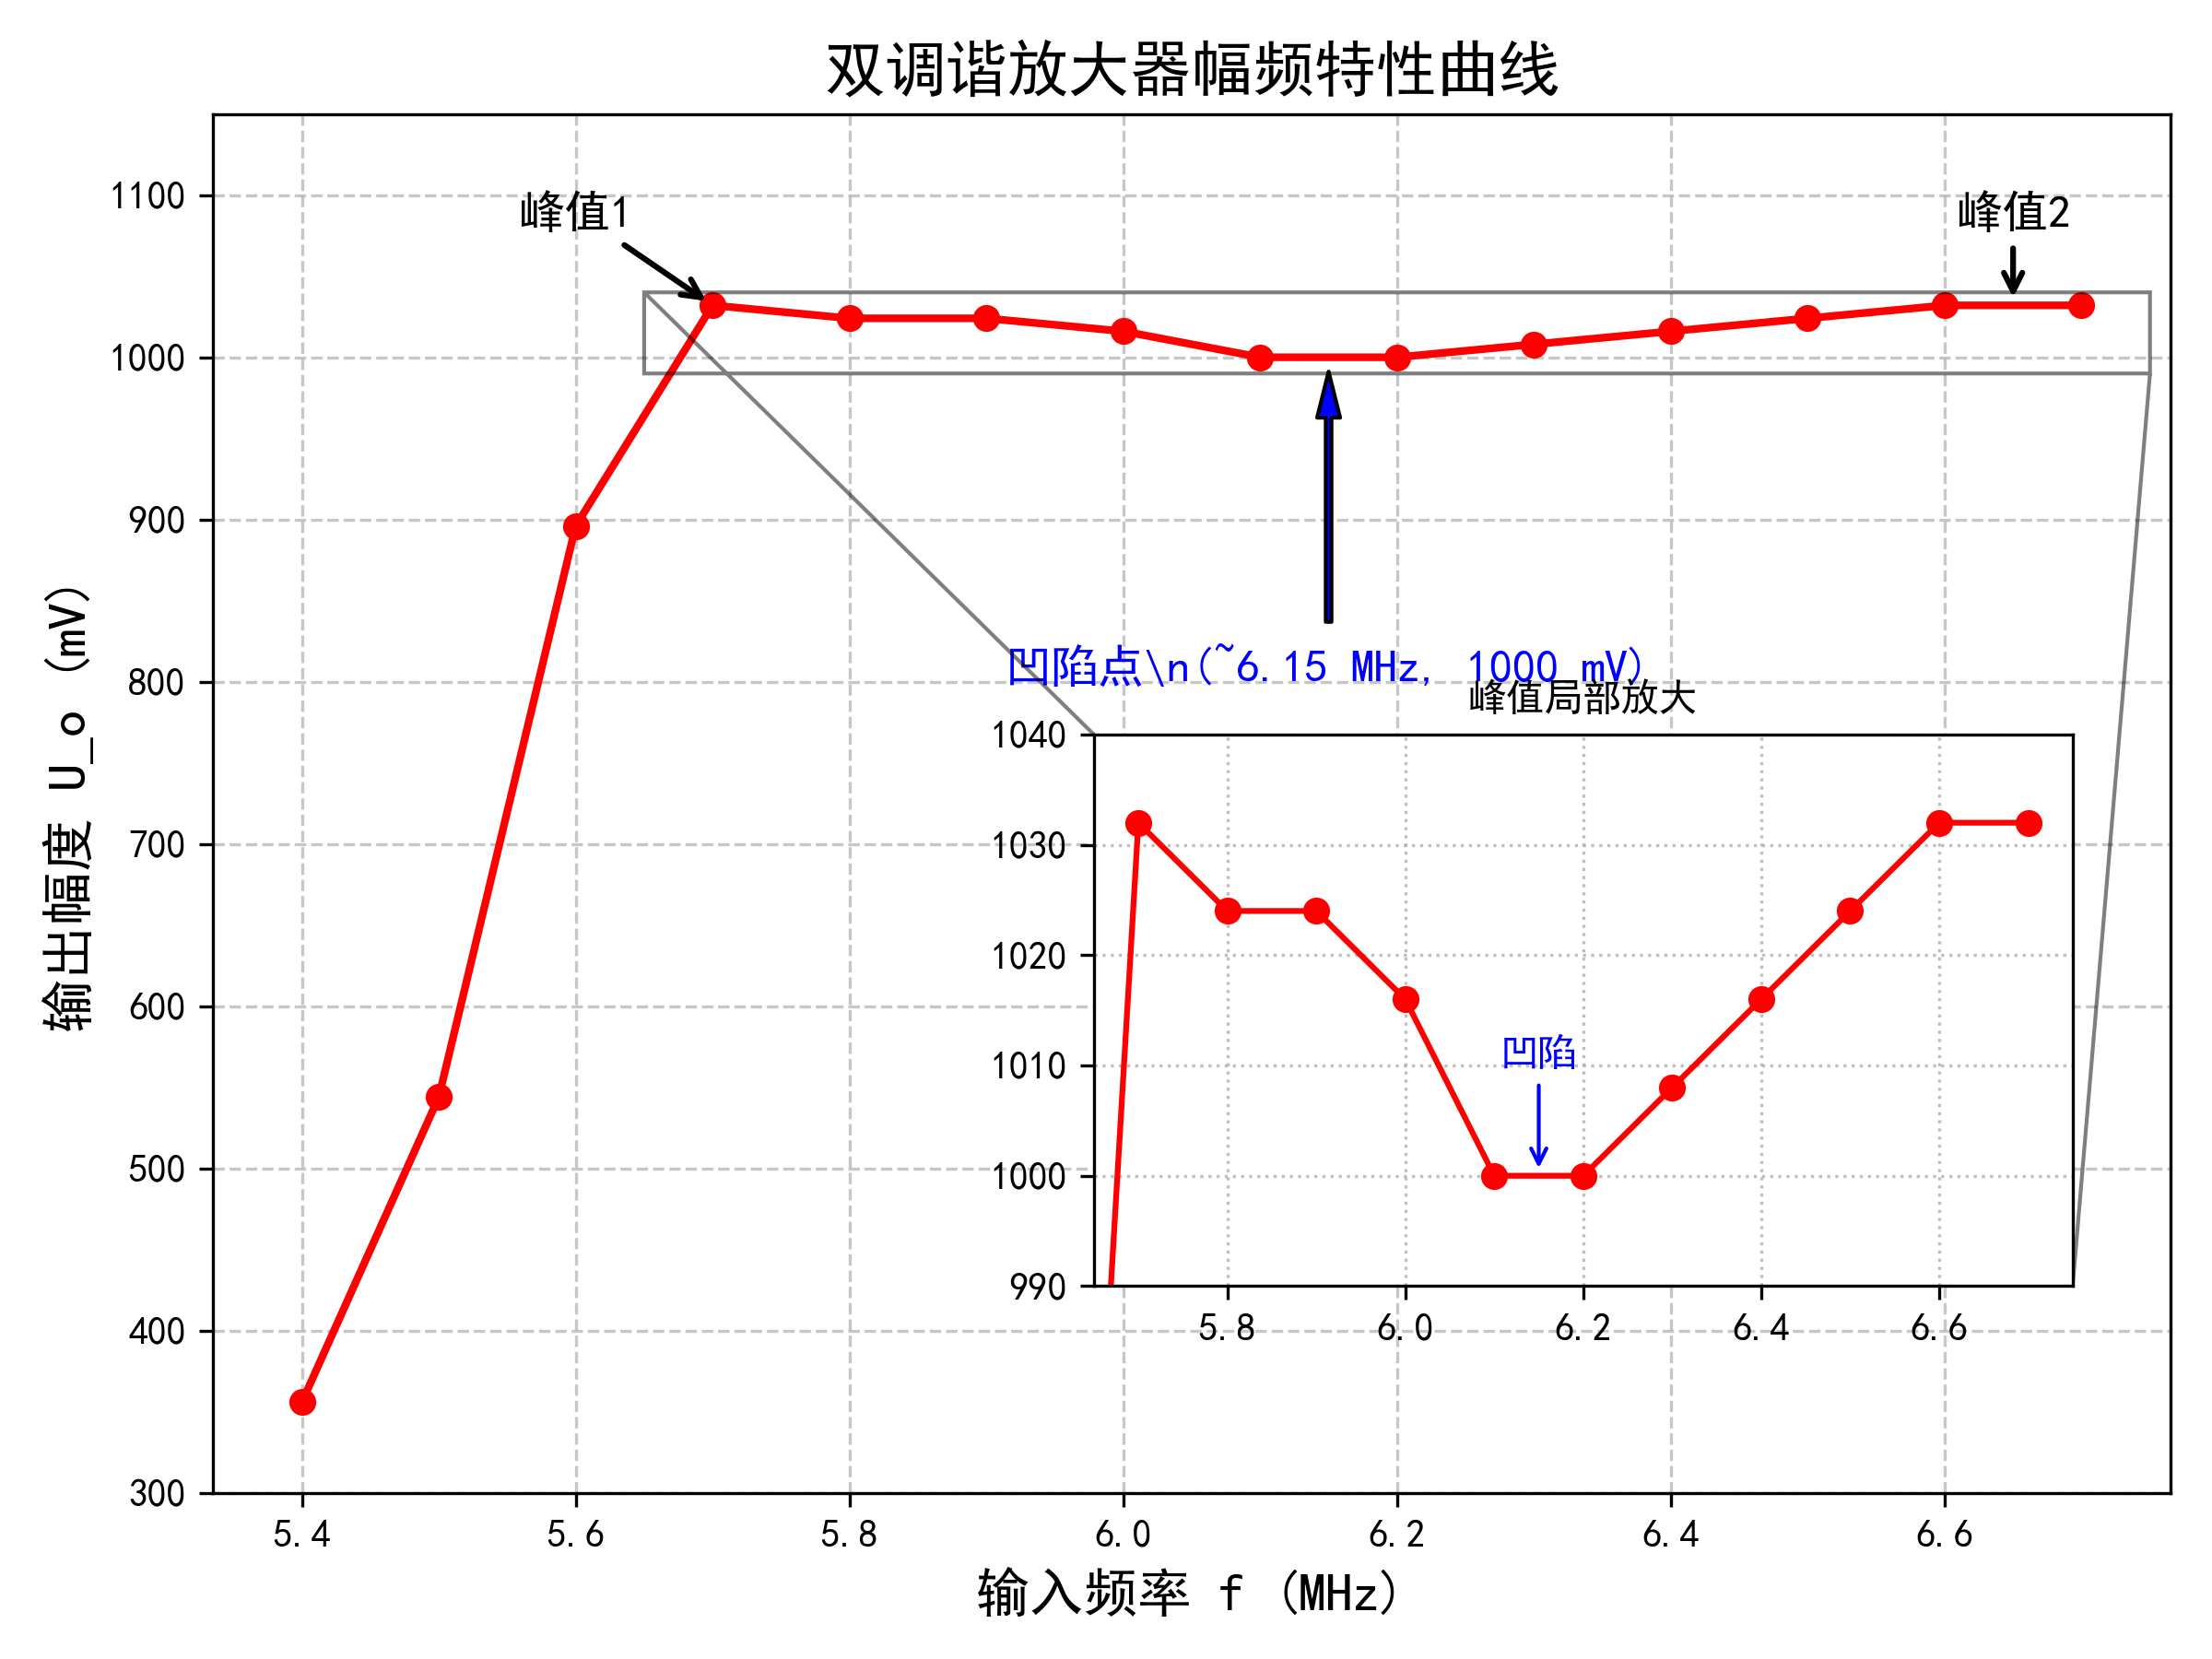
\includegraphics[width=0.8\textwidth]{双调谐幅频特性曲线.png}
    \caption{双调谐放大器幅频特性曲线}
    \label{fig:double_tuned_curve_new}
    \end{figure}
    \item[d.] \textbf{耦合电容 1C19 对特性的影响}：通过调整 1C19 的容量，观察到耦合程度的变化会显著改变曲线的形状（单峰、平顶或双峰）。以下为扫频曲线对比：
\end{itemize}

% 预留并列三栏图片
\begin{figure}[H]
    \centering
    \begin{minipage}[t]{0.32\textwidth}
        \centering
        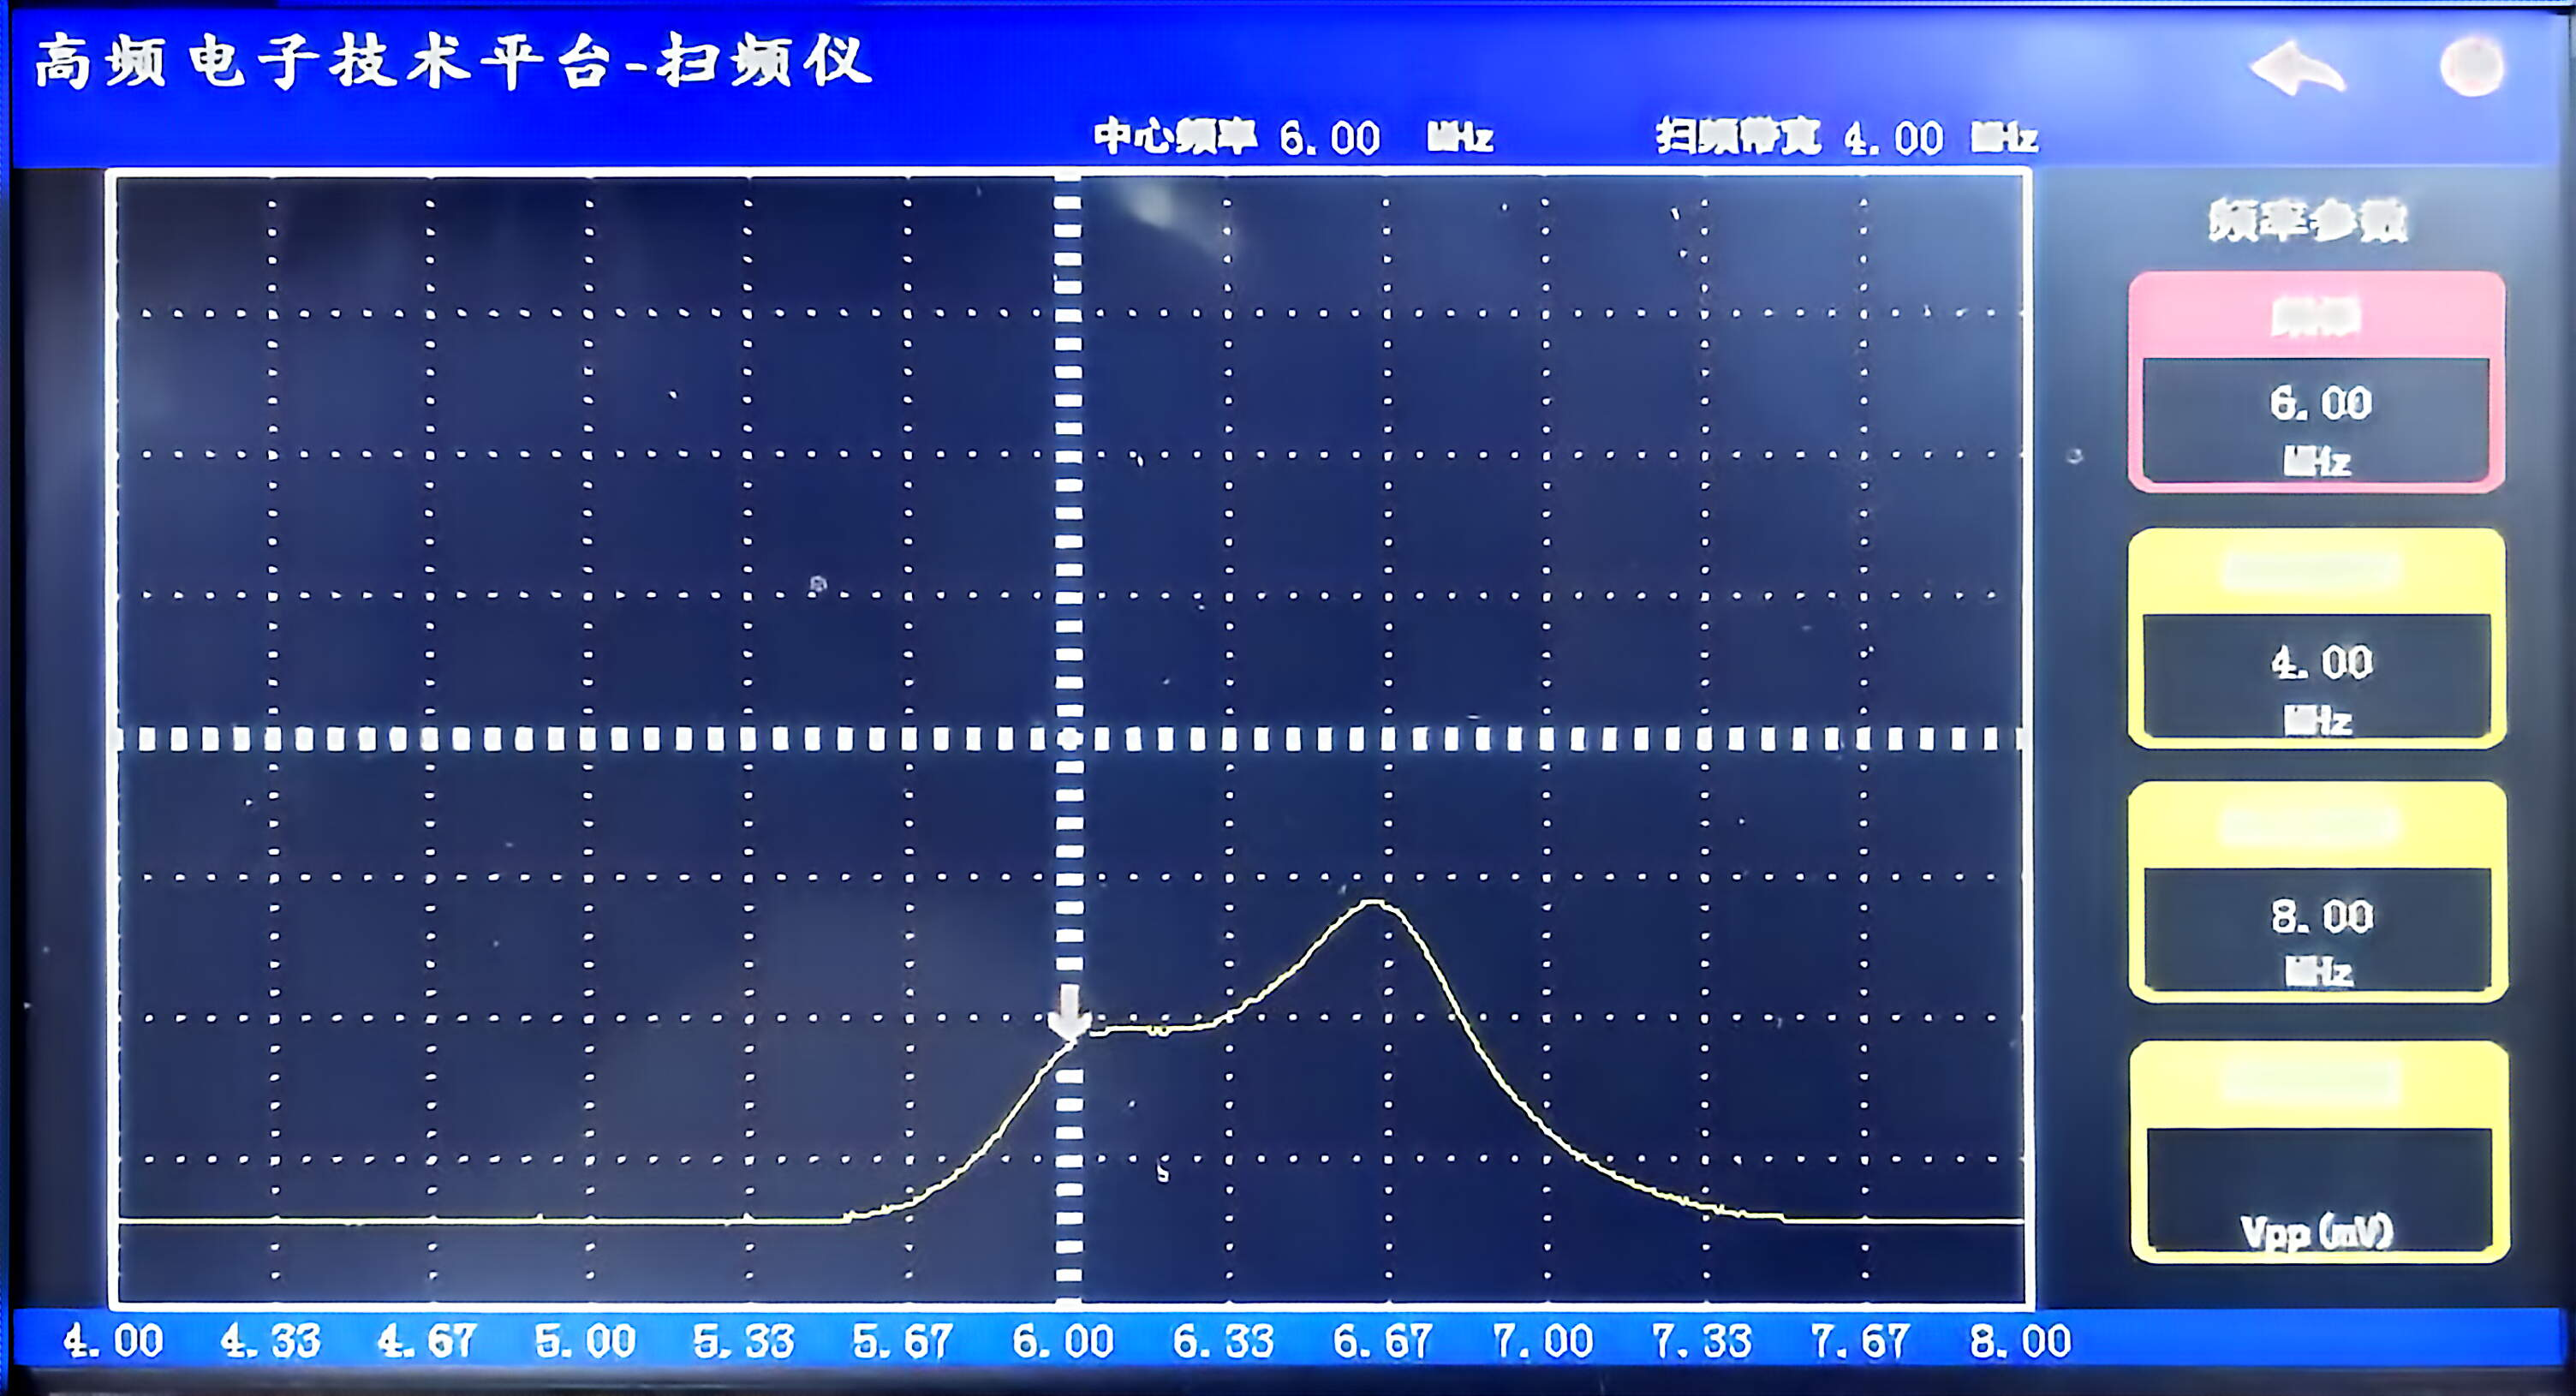
\includegraphics[width=\textwidth, height=3.5cm]{耦合电容减小扫频曲线.jpg} % 替换为：耦合电容减小.jpg
        \caption{耦合电容减小扫频曲线}
    \end{minipage}
    \hfill
    \begin{minipage}[t]{0.32\textwidth}
        \centering
        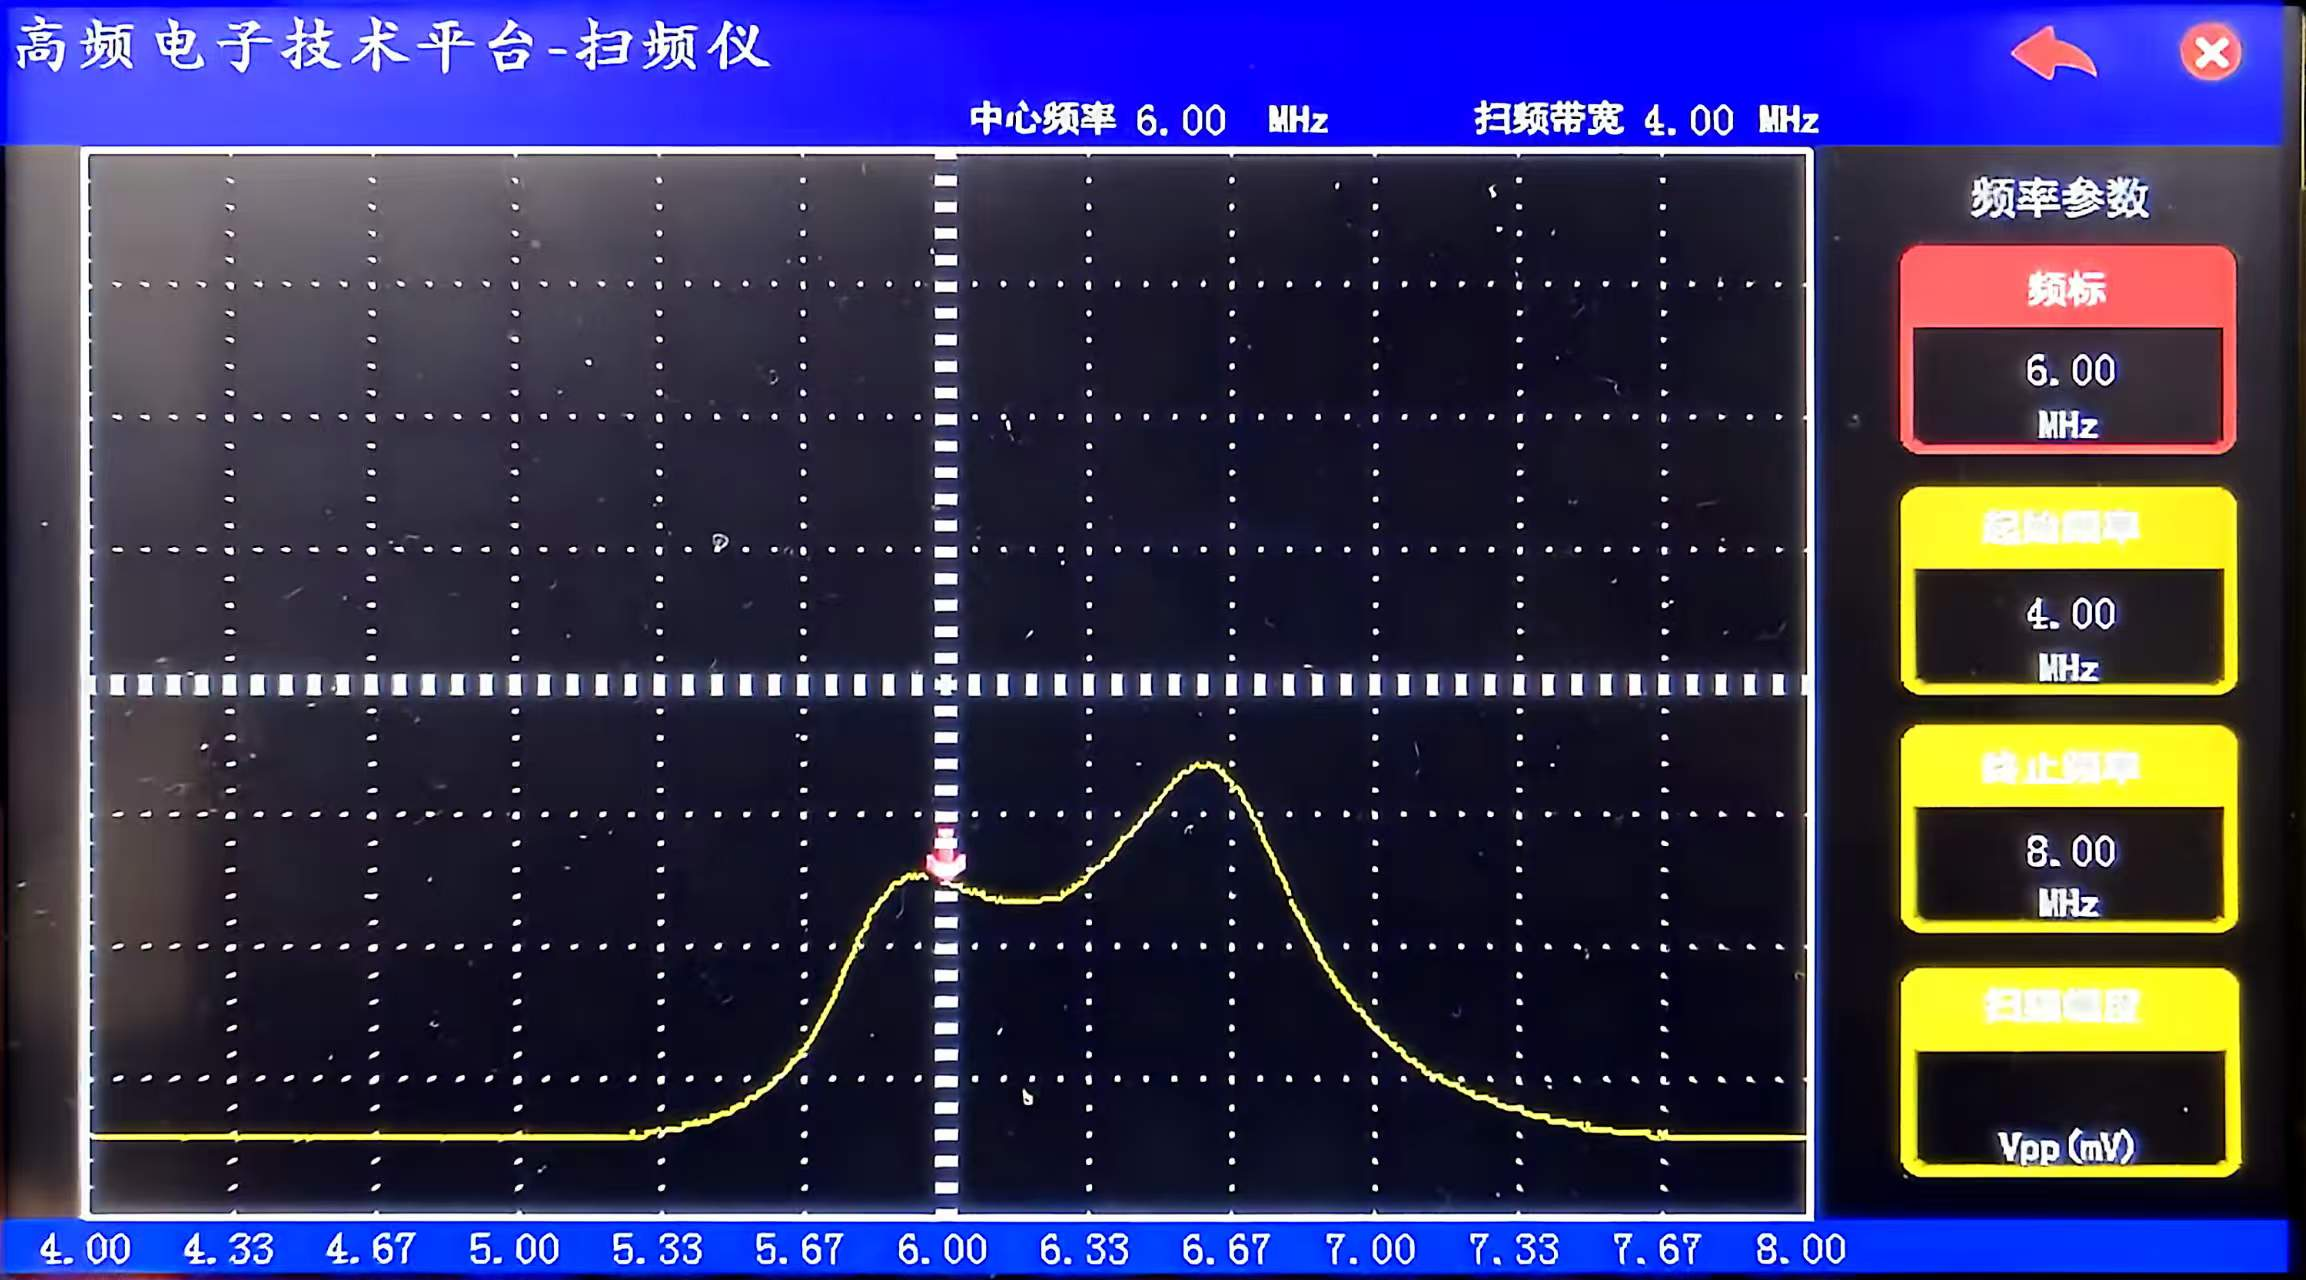
\includegraphics[width=\textwidth, height=3.5cm]{耦合电容 1C19 为某一值时扫频曲线.jpg} % 替换为：1C19为某值.jpg
        \caption{耦合电容 1C19 为某一值时扫频曲线}
    \end{minipage}
    \hfill
    \begin{minipage}[t]{0.32\textwidth}
        \centering
        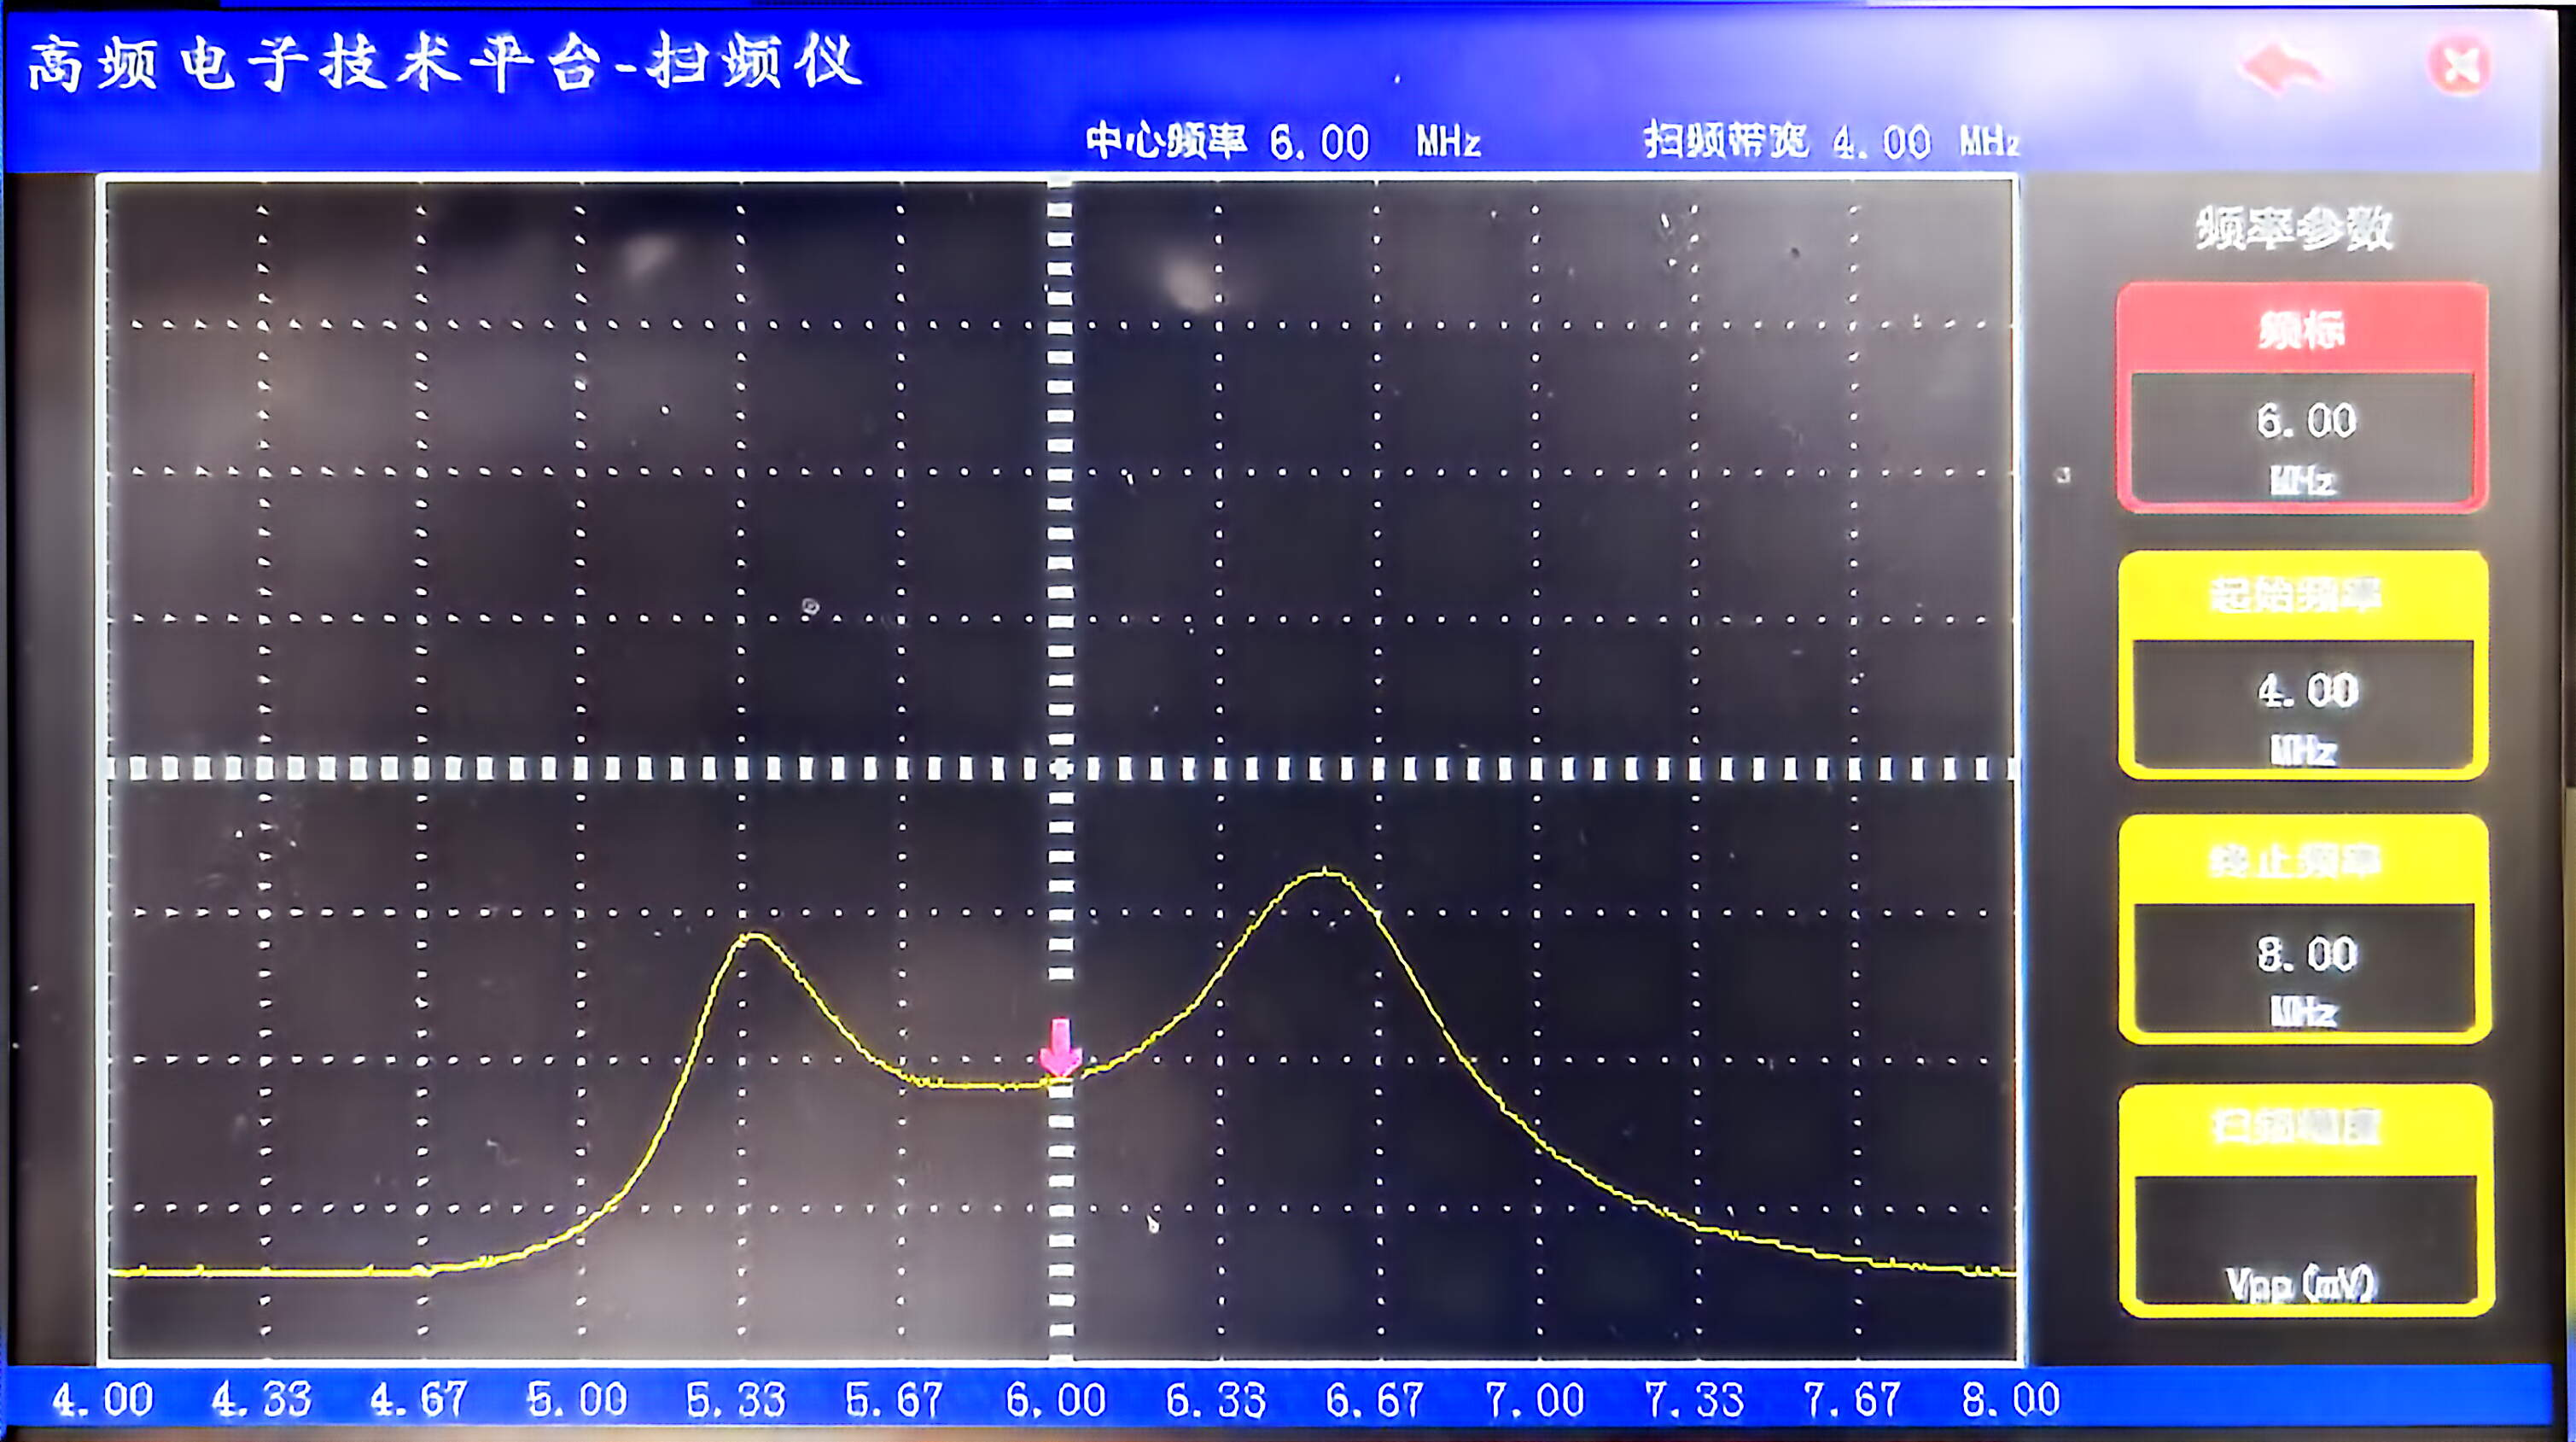
\includegraphics[width=\textwidth, height=3.5cm]{耦合电容增大扫频曲线.jpg} % 替换为：耦合电容增大.jpg
        \caption{耦合电容增大扫频曲线}
    \end{minipage}
    \vspace{0.5em}
    \caption{不同 1C19 耦合情况下的幅频特性扫频曲线对比}
\end{figure}

\subsubsection*{2. 结果分析}

\textbf{测试数据特征分析：}
\begin{itemize}
    \item \textbf{双调谐峰谷特征：} 表格数据呈现出经典的“双峰”现象。随着频率变化，在 $5.7\text{MHz}$ 与 $6.6 \sim 6.7\text{MHz}$ 周边均达到了峰值 $1032\text{mV}$。而在它们之间的区域输出出现下凹，测出两峰之间凹陷点的频率约为 $6.15\text{MHz}$（跌至约 $1000\text{mV}$）。出现清晰的双峰和凹凸交替表明当前的两级谐振回路处于“过耦合”状态。
    \item \textbf{选择性较单调谐优良：} 相比于单调谐电路，双调谐在横跨 $5.7\text{MHz}$ 到 $6.7\text{MHz}$ 的极宽频带域内，输出幅度持续平坦地保持在 $1000\text{mV}$ 以上。它对带内信号的增益平坦度远超单调谐；同时在边缘（如 $5.4\text{MHz}$ 径直跌向 $356\text{mV}$）的滚降极为陡峭，矩形系数更小。
\end{itemize}

\subsection*{任务四：放大器动态范围测量}

为测量放大器的动态范围边界，将系统恢复为单调谐配置状态，即将开关1K1置于“断开”状态，同时将开关1K2置于“接通”状态。调节高频信号源，将其频率固定在放大器的空载谐振中心频率6.3MHz处，并为了不引起失真将初始输入幅度微调设定为150mV（此时同样由示波器CH1通道进行严密监控）。

幅度扫描测试操作：按照预设的观察表格步长，逐步且缓慢地增加高频源的输出电压幅度，驱动输入幅度从150mV逐渐攀升至极端的500mV，并在每一个规定的幅度检验点处，通过示波器CH2通道准确读出对应的放大端输出电压峰峰值。

实时记录以计算每一个数据点电压输入输出间的电压放大倍数规律，关注示波器上显示的终态输出波形的非线性变化。当发现波形不再是标准正弦波，而出现顶部削平或底部畸变等典型的三极管饱和及截止导致的大信号失真现象时，即找到了该小信号谐振放大器工作的最大动态幅度限值。

\subsubsection*{1. 测试结果}

\begin{table}[H]
\centering
\label{tab:dynamic_range_results}
\begin{tabular}{c*{10}{c}}
\toprule
放大器输入 (mV) & 150 & 180 & 194 & 230 & 250 & 280 & 310 & 350 & 400 & 500 \\
\midrule
\textbf{放大器输出 (V)} & - & - & 1.380 & 1.560 & 1.740 & 1.860 & 2.080 & 2.360 & 2.520 & 3.020 \\
\textbf{电压放大倍数} & - & - & 7.11 & 6.78 & 6.96 & 6.64 & 6.71 & 6.74 & 6.30 & 6.04 \\
\bottomrule
\end{tabular}
\caption{放大器动态范围测试结果}
\end{table}

 \begin{figure}[htbp]
 \centering
 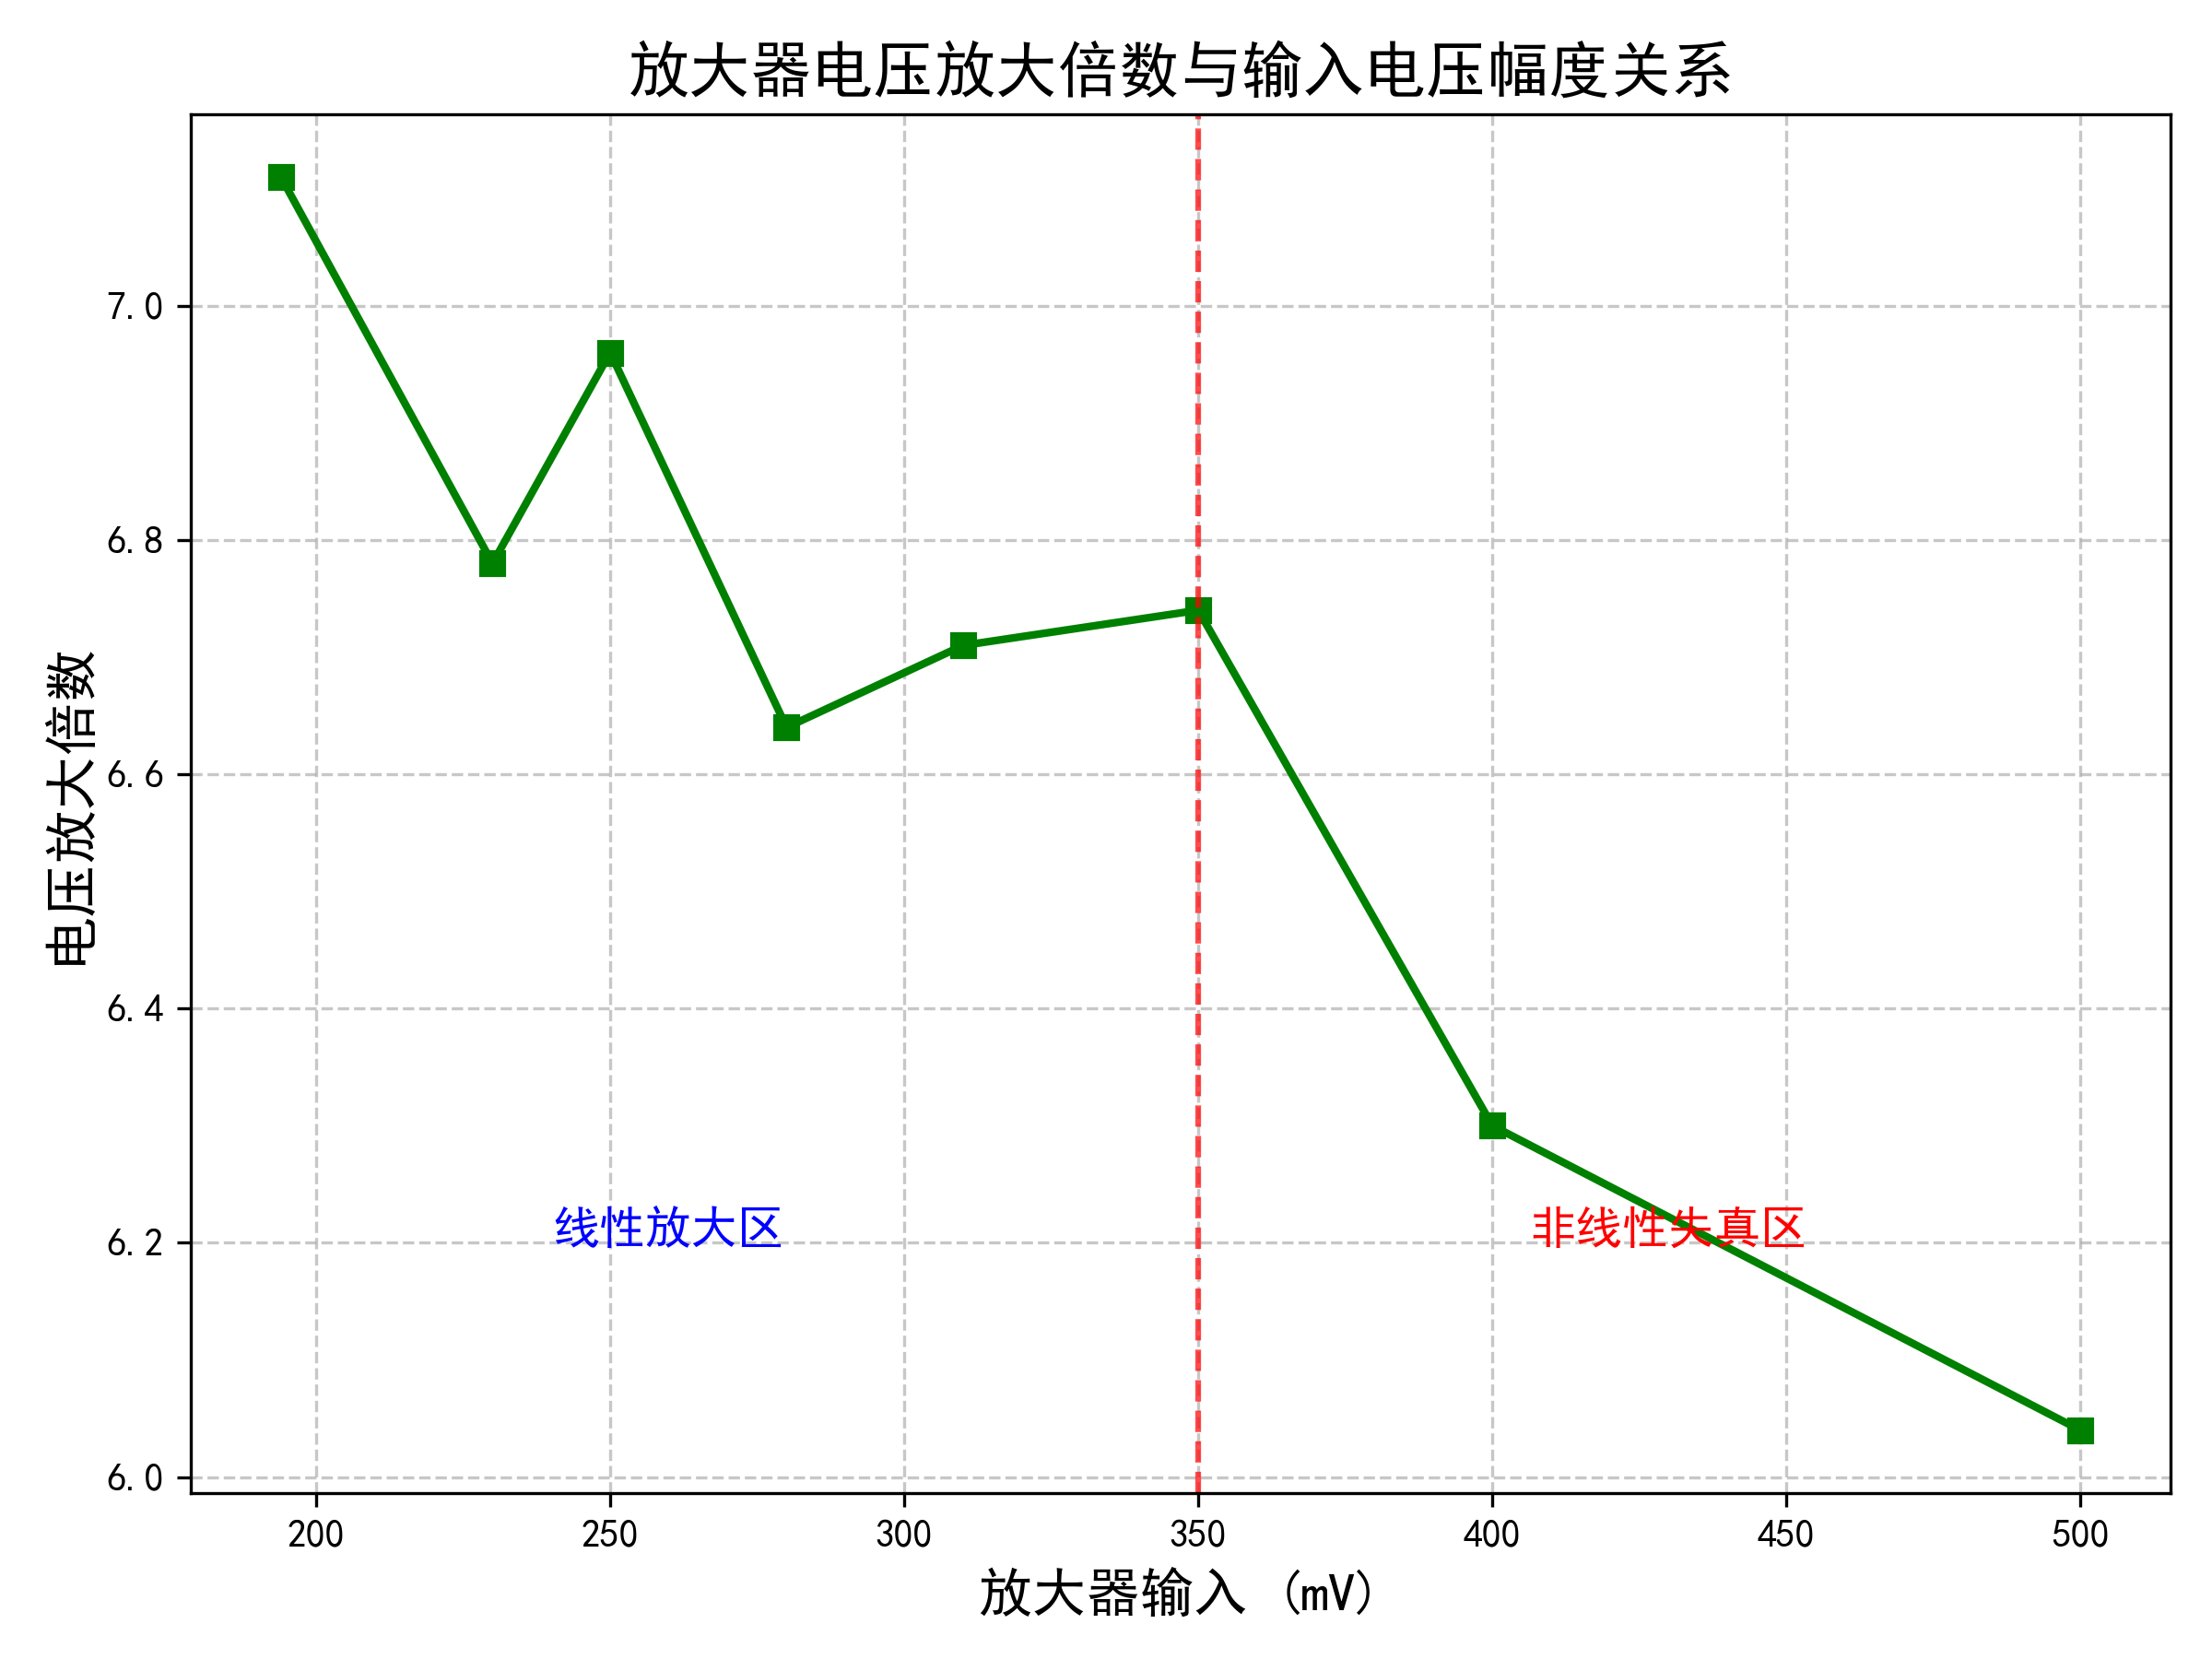
\includegraphics[width=0.8\textwidth]{放大器动态范围曲线.png}
 \caption{放大器动态范围曲线}
 \label{fig:dynamic_range_curve}
 \end{figure}

\subsubsection*{2. 结果分析}

\textbf{测试数据及失真阶段分析：}
\begin{itemize}
    \item \textbf{线性动态范围分析：} 观察测试结果可知，在小信号输入阶段（$U_{in}$ 为 $194\text{mV} \sim 350\text{mV}$ 时），晶体管基本工作在伏安转移特性的线性放大区内，输出电压和输入电压呈现出良好成比例放大的关系，测到的电压放大倍数 $A_v$ 极其平稳地维持在 $6.64 \sim 7.11$ 的有限区间波动。
    \item \textbf{失真与非线性特征：} 当输入信号幅度继续增强、推进至 $400\text{mV}$ 甚至 $500\text{mV}$ 时，虽然放大器输出幅度依然被迫走高，但“电压放大倍数”这一硬性指标明显跌落至 $6.30$ 乃至 $6.04$。放大倍率衰退意味着由于输入信号过载，晶体管已受输入压强推拉进入饱和区或截止区。过大的输入幅度打破了小信号的基准假设，波形产生了极其典型的削顶等大信号非线性失真。总结而言，当前该系统的安全线性动态绝对边界约为 $350\text{mV}$ 左右。
\end{itemize}

\section*{四. 总结}

本次《小信号调谐放大器》实验，让我对高频电子线路中调谐放大器的工作原理有了更深刻和直观的认识。

单调谐回路虽然结构简单、容易调节，且谐振点处增益高，但其选择性相对一般，通频带不够理想；相比之下，双调谐回路利用耦合电容将初次级回路相连，在合适的临界或弱过耦合状态下能够实现通频带顶部平坦、边缘下降更陡峭的优良特性（具有更小的矩形系数），这对于需要兼顾较宽频带与相邻窄带干扰抑制的通信接收机更具有现实应用价值。

在电路参数对高频放大器性能影响的探究中，扫频仪让我对集电极负载和耦合电容对高频性能的影响有了直观的体会。接通开关并入负载电阻，回路等效负载变小导致回路自身有效品质因数 $Q$ 值降低，此时物理现象直接表现为幅频特性曲线变“胖”、通频带展宽且中心谐振最大增益出现大幅度的下降。双调谐实验中，改变耦合电容的值能明显引起双峰凹陷和峰值间距的位移变换，“临界耦合”对于获得理想单峰也有较大的作用。此外，动态范围测试捕捉到了当输入信号幅度过大导致三极管进入非线性区域后引起的严重的高频波形削顶失真。

本次实验让我对高频信号源发生器、双通道示波器以及成型高频实验平台的操作都有了更深的了解。在寻找谐振点极值幅度跳变和测量高频微弱信号时，仪器读数随线缆抖动波动以及受环境高频噪声轻微干扰，通过仔细调节系统稳压触发电平、稳固探头与主板连线接地以及保持规范调节旋钮的细小步长控制等有效举措，才能提取出稳定有效的数据源。

\end{document}